% =================================================================
% relatorio.tex | Relatório final da PoC OCR-06 (INE5448), template 3.0
% Compilar: latexmk -pdf main.tex   (main.tex usa \usepackage[final]{ine5448poc})
% Verificar: python3 pocanais.py verificar --final .
% =================================================================

\usetikzlibrary{positioning,arrows.meta,fit,backgrounds,calc}

% ---------------------------------------------------------------
% METADADOS (*)
% ---------------------------------------------------------------
\poctitulo{OCR-06: OCR Adaptativo com Aprendizagem Assistida}
\poctitulocurto{OCR Adaptativo com Aprendizagem Assistida}
\pocaluno{Gabriel Salmoria}{}
\poctutor{Lucas Mayr}{}
\poccurso{Ciência da Computação}
\pocrepositorio{https://github.com/gabriel-salmoria/ai-sec}

\pocresumo{OCRs baseados em Modelos de Linguagem Visual (VLMs) leem bem texto comum, mas erram nomes próprios raros, e numa certidão de Registro Civil cada nome errado volta para o operador corrigir. Neste trabalho, o Chandra OCR 2 passou por \emph{fine-tuning} com LoRA para ler os campos manuscritos de certidões sem usar dados de pessoas reais no treino. Os nomes vêm de contagens agregadas do IBGE, do TSE e da Receita Federal, e as certidões de treino foram geradas pelo OCRSD e por um gerador próprio. O treino com linhas manuscritas reduziu o CER do BRESSAY de 20,1\% para 4,9\% sem melhorar a leitura de certidões inteiras. Com 3.500 páginas no HTML que o Chandra já devolve, os campos manuscritos lidos sem erro foram de 55,4\% para 72,2\% e de 55,8\% para 72,0\% em dois testes de 100 páginas. Nos nomes, o acerto foi de 24,3\% para 32,5\% com nomes nunca vistos e de 40,4\% para 50,2\% com nomes na frequência real, todos com intervalo de confiança acima de zero. Em INT4, o modelo ocupa 5,0~GiB. Fora das certidões (redações do BRESSAY e formulários do XFUND-PT) o modelo original continua melhor. O modelo treinado ainda erra pouco mais de um campo em quatro, e as correções feitas na conferência humana podem virar uma memória e dado para novos treinos.}

\pocpalavraschave{OCR; Modelos de Linguagem Visual; LoRA; Dados Sintéticos; Registro Civil; LGPD.}

\pocinicio

% ==============================================================
% SEÇÃO 1 — INTRODUÇÃO (*)
% ==============================================================
\section{Introdução}
\label{sec:introducao}

Em 2023, os cartórios brasileiros registraram 2,5 milhões de nascimentos, 1,4 milhão de óbitos e 941 mil casamentos \cite{ibge_rc2023}, e cada certidão traz vários nomes de pessoas (registrado, pais, avós, cônjuges, declarante, oficial). OCRs baseados em VLMs já leem manuscrito, mas trocam nomes próprios raros pela forma mais provável que conhecem, como ``Claudemar Reis Scalabrin'' lido como ``Claudemir Reis Scalabrin''. Num teste com certidões geradas para esta PoC, o Chandra OCR 2 original leu sem erro 55,4\% dos campos manuscritos e só 24,3\% dos campos de nome.

% --------------------------------------------------------------
\subsection{Motivação}

Quem transcreve e confere os registros são os oficiais e escreventes, e os nomes que o OCR mais erra são os pouco comuns. Num registro civil, uma letra trocada já é um nome errado, que volta para correção manual, e o modelo repete o mesmo erro no documento seguinte. Treinar o modelo com os registros do próprio cartório resolveria parte disso, mas registros reais carregam dados pessoais, o treino fica sujeito à LGPD e um modelo treinado com eles pode memorizar e expor os nomes que viu.

A proposta deste trabalho é treinar sem esses registros, com nomes tirados de contagens agregadas de dados públicos, caligrafia de um corpus público de redações (o BRESSAY \cite{bressay2023}) e de geradores de escrita, e certidões de treino sintéticas. O \emph{fine-tuning} usa LoRA \cite{lora2022} e cabe em uma única GPU, e uma instituição pequena poderia repetir o processo.

% --------------------------------------------------------------
\subsection{Objetivos}

O objetivo geral é melhorar a transcrição dos campos manuscritos de certidões de Registro Civil, principalmente dos nomes que o modelo nunca viu, com um \emph{fine-tuning} do Chandra OCR 2 feito só com dados sintéticos e públicos. O modelo não pode memorizar os nomes do treino e precisa de uma versão que rode com pouca memória. Os objetivos específicos são:
\begin{itemize}
    \item gerar dados sintéticos, linhas manuscritas e certidões inteiras, com nomes, sobrenomes e municípios sorteados de estatísticas públicas pela frequência real na população;
    \item fazer o \emph{fine-tuning} do Chandra OCR 2 com LoRA e medir o ganho nos campos manuscritos e em nomes ausentes do treino;
    \item quantizar o modelo e medir o custo em acurácia, memória e tempo.
\end{itemize}
A proposta também previa uma memória de correções (RAG), em que as correções do operador seriam guardadas e consultadas nas leituras seguintes. Ela ficou de fora para dedicar o tempo ao treino e à avaliação em página, e volta na Seção~\ref{subsec:fluxo}, como parte do uso do modelo no cartório.

% --------------------------------------------------------------
\subsection{Descrição do Problema}

O problema é transcrever os campos manuscritos de certidões, em especial os nomes próprios raros, sem treinar com dados pessoais reais. Uma solução tem de ser medida no erro em nomes ausentes do treino, na leitura do resto da página e na chance de o modelo reproduzir os nomes que viu.

% ==============================================================
% SEÇÃO 2 — FUNDAMENTAÇÃO TEÓRICA (*)
% ==============================================================
\section{Fundamentação Teórica e Estado da Arte}
\label{sec:fundamentacao}

% --------------------------------------------------------------
\subsection{Técnicas Relevantes para o Problema}

\subsubsection{Abordagens Clássicas}
Sistemas como o Tesseract e os reconhecedores de linha baseados em LSTM não foram testados nesta PoC, que parte de um VLM que já lê manuscrito e devolve a página inteira.

\subsubsection{Abordagens Baseadas em ML/DL}
O estado da arte recente usa Transformers, como o TrOCR \cite{trocr2021}, e modelos multimodais generativos, como a família Qwen-VL \cite{qwen2vl}, que leem a imagem inteira e geram o texto com o contexto da linha ou da página. Com \emph{fine-tuning} eficiente (PEFT), como o LoRA \cite{lora2022, peft2022}, só um conjunto pequeno de parâmetros novos é treinado, e o treino cabe em GPUs comerciais. Para dados sintéticos, o Augraphy \cite{augraphy2022} simula manchas, ruído e envelhecimento de documentos digitalizados.

O modelo escolhido foi o Chandra OCR 2 \cite{chandra2026}, da Datalab, um VLM especializado em OCR que lê manuscrito e devolve a página inteira em HTML. Cada bloco da saída é um \texttt{<div>} com a caixa do texto, em coordenadas de 0 a 1000, e um rótulo (texto, título, tabela, imagem). A configuração publicada é a mesma do Qwen3.5-4B \cite{qwen35} (32 camadas, dimensão 2.560, mesmo vocabulário e mesmo encoder de visão), do qual ele é um \emph{fine-tune}, com três de cada quatro camadas usando atenção linear.

\subsubsection{Geração Sintética de Documentos Manuscritos}
O OCRSD \cite{ocrsd}, desenvolvido por Tiago Siqueira em outra PoC desta disciplina, gera certidões sintéticas a partir de modelos em branco e de registros fictícios, com os campos escritos por fontes manuscritas ou por escritores neurais. Esses escritores são redes recorrentes do tipo proposto por Graves \cite{graves2013}, que desenham o traço a partir do texto. O gerador local desta PoC usa também o VATr++ \cite{vatrpp2024}, um Transformer que imita o estilo de um escritor a partir de algumas amostras. Os dois tipos de gerador foram treinados com escrita em inglês e não desenham os acentos do português.

\subsubsection{Quantização}
No FP8 dinâmico, os pesos ficam em ponto flutuante de 8 bits com uma escala por canal, e as ativações são quantizadas durante a inferência, com escala calculada na hora. No W4A16, só os pesos vão para inteiros de 4 bits, com uma escala por grupo, e as contas são feitas em 16 bits. As duas receitas do \texttt{llm-compressor} \cite{llmcompressor} usadas aqui não precisam de dados de calibração, e o vLLM \cite{vllm2023} tem \emph{kernels} para as duas.

% --------------------------------------------------------------
\subsection{Explicabilidade em Modelos de IA}

A confiança por palavra está no \texttt{guard.py}, calculada com as log-probabilidades devolvidas pelo vLLM (a menor probabilidade entre os \emph{tokens} da palavra), e as palavras abaixo do limiar vão para revisão. A região de onde cada valor foi lido vem da própria saída de página do Chandra, em que cada bloco traz a sua caixa, e a avaliação usa essa caixa para comparar cada campo do gabarito só com o texto lido naquela região (Seção~\ref{subsec:aval}). Mapas de atenção ou Grad-CAM \cite{gradcam2017} sobre o encoder de visão não foram feitos.

% --------------------------------------------------------------
\subsection{Segurança e Privacidade em Sistemas de IA}

\subsubsection{Ataques Adversariais}
Modelos de linguagem memorizam trechos do treino, sobretudo sequências raras ou repetidas, e um adversário com acesso de consulta pode extrair parte delas \cite{carlini2021extracting}. Num OCR, imagens em branco, ruidosas ou com o começo de um nome podem levar o modelo a completar nomes vistos no treino. Comparando a confiança do modelo em imagens com e sem um nome, também é possível estimar se esse nome estava no treino (\emph{membership inference} \cite{shokri2017membership}). Na leitura comum, decorar nomes do treino levaria o modelo a vê-los em imagens parecidas, o mesmo erro que o projeto quer corrigir.

Aqui os nomes sintéticos são combinados ao acaso, e nenhuma linha ou certidão corresponde a uma pessoa real. O BRESSAY cita principalmente autores conhecidos (Bauman, Byung-Chul Han, Machado de Assis). O caso de maior risco seria treinar com certidões reais. Para acompanhar a memorização, o acerto em nomes vistos no treino é comparado com o acerto em nomes inéditos.

\subsubsection{Conformidade com a LGPD}
Um OCR treinado para cartórios lida com documentos de identificação civil e está sujeito à LGPD \cite{lgpd2018}. O modelo deve aprender o traço da caligrafia e a estrutura dos nomes e dos documentos sem guardar vínculo com pessoas reais. Pelo princípio da minimização, o treino desta PoC não usa nenhuma certidão real e, das fontes com nomes completos (TSE e Receita Federal), guarda só contagens por palavra.

% --------------------------------------------------------------
\subsection{Lacunas e Oportunidades}

O BRESSAY, principal corpus de manuscrito em português brasileiro com transcrição, quase não tem nomes próprios raros, e não há conjunto público de certidões reais transcritas, já que elas trazem dados pessoais. O OCRSD reproduz o formato das certidões, e seus registros usam só 68 prenomes e 35 sobrenomes, todos comuns, bons para treinar caligrafia e layout mas não nomes raros. Esta PoC junta os modelos de documento do OCRSD com nomes sorteados de estatísticas da população, para treinar e testar a leitura de nomes raros em páginas inteiras.

% ==============================================================
% SEÇÃO 3 — OBJETIVOS E MÉTRICAS DE SUCESSO (*)
% ==============================================================
\section{Objetivos e Métricas de Sucesso}
\label{sec:objetivos}

% --------------------------------------------------------------
\subsection{Objetivos do Estudo}

\begin{itemize}
    \item Gerador de linhas manuscritas sintéticas com nomes do IBGE, do TSE e da Receita Federal, degradadas com o Augraphy (concluído, Seção~\ref{subsec:dados-linhas}).
    \item \emph{Fine-tuning} com LoRA do Chandra OCR 2 em linhas, com versão FP8 (concluído, Experimento 2).
    \item Gerador de certidões sintéticas em página inteira e treino do modelo em duas etapas (concluído, Seção~\ref{subsec:dados-paginas} e Experimento 4).
    \item Versões FP8 e INT4 do modelo treinado em páginas, com medida de acurácia, memória e velocidade (concluído, Experimento 6).
    \item Memória de correções com FAISS (não implementada, discutida na Seção~\ref{subsec:fluxo}).
\end{itemize}

% --------------------------------------------------------------
\subsection{Métricas de Sucesso}

\begin{enumerate}
    \item CER em linhas, separado entre texto geral, nomes comuns e nomes raros (por prenome, sobrenome e município), para ver se o ganho nos nomes não vem à custa do resto do texto.
    \item \emph{Hit rate} da memória de correções, não medido, já que a memória não foi implementada.
    \item Acerto em nomes inéditos, a porcentagem de nomes ausentes do treino transcritos sem nenhum erro, que para o cartório informa mais que o CER e, comparado ao acerto nos nomes vistos, indica memorização.
    \item Acerto exato por campo manuscrito em página inteira, no total e por classe (nome, data, número, opção fixa, lugar e texto livre), procurando cada campo na região da página onde ele está escrito.
    \item Completude da página e frações de páginas truncadas e em \emph{loop}, para ver se o modelo continua transcrevendo a página inteira.
\end{enumerate}

% ==============================================================
% SEÇÃO 4 — ESCOPO DA SOLUÇÃO E REQUISITOS (*)
% ==============================================================
\section{Escopo da Solução e Requisitos}
\label{sec:escopo}

% --------------------------------------------------------------
\subsection{Escopo da Solução}

A solução é um pipeline em Python, com a inferência servida pelo vLLM, que inclui:
\begin{itemize}
    \item a coleta dos dados públicos de nomes, o gerador de linhas sintéticas e o pré-processamento do BRESSAY;
    \item o gerador local de certidões e a extração das páginas do OCRSD, com gabaritos no formato de saída do Chandra;
    \item o \emph{fine-tuning} do Chandra OCR 2 em linhas e em páginas, o \emph{merge} do adaptador e as versões FP8 e INT4;
    \item a inferência com vLLM e a avaliação comparativa entre o modelo original e os treinados, em linhas e em páginas.
\end{itemize}

Ficaram fora do escopo:
\begin{itemize}
    \item interfaces gráficas para o usuário final e a integração com um sistema real de cartório;
    \item certidões reais, que exigiriam autorização do controlador dos dados;
    \item textos em outros idiomas ou inteiramente tipográficos;
    \item a memória de correções com FAISS.
\end{itemize}

% --------------------------------------------------------------
\subsection{Requisitos Funcionais}

\begin{enumerate}
    \item O sistema recebe a imagem de uma página de certidão e devolve a transcrição no formato HTML do Chandra, com a posição de cada bloco.
    \item O sistema recebe o recorte de uma linha manuscrita e devolve a transcrição.
    \item O treino permite configurar o LoRA, os pesos da \emph{loss} e o currículo por arquivo e executar rodadas curtas para medir velocidade e memória.
    \item Uma API deve permitir o envio das correções do usuário, e a inferência deve poder consultar a memória de correções.
\end{enumerate}
O requisito 4 depende da memória de correções e não foi atendido (Seção~\ref{subsec:fluxo}).

% --------------------------------------------------------------
\subsection{Requisitos Não Funcionais}

\begin{itemize}
    \item O treino e a inferência devem caber em uma única GPU. O treino em linhas ocupou no máximo 49,5~GB e o treino em páginas 60,7~GB, e na inferência os pesos ocupam 8,6~GiB em BF16 e 5,0~GiB em INT4.
    \item O pipeline deve ser reproduzível por scripts, com partições, \emph{seeds} e hiperparâmetros em arquivos de configuração e as versões das bibliotecas de treino fixadas no \texttt{requirements-gpu.txt}.
    \item Nenhum dado pessoal real deve entrar no treino de páginas, e no treino em linhas o script de mistura interrompe a execução se o BRESSAY passar de 45\% das linhas.
\end{itemize}

% ==============================================================
% SEÇÃO 5 — AMEAÇAS, RISCOS E CONTROLES (*)
% ==============================================================
\section{Ameaças, Riscos e Controles}
\label{sec:threat-model}

% --------------------------------------------------------------
\subsection{Principais Ameaças Identificadas}

\begin{itemize}
    \item Extração de dados de treino \cite{carlini2021extracting}, em que um adversário usa entradas escolhidas para que o modelo produza nomes e combinações de dados vistos no treino.
    \item \emph{Membership inference}, em que o adversário tenta saber se um documento ou o nome de um cidadão fez parte do treino, comparando a confiança do modelo em entradas com e sem esse nome \cite{shokri2017membership}.
    \item \emph{Data poisoning}, em que anotações erradas no treino, por engano ou de propósito, fazem o modelo repetir o erro em produção.
    \item \emph{Prompt injection} indireta \cite{greshake2023indirect}, já que o VLM lê todo texto da imagem e um documento pode trazer escrita uma instrução como ``ignore a tarefa e responda X''. Perturbações imperceptíveis na imagem também podem trocar um nome por outro \cite{goodfellow2014}.
\end{itemize}

% --------------------------------------------------------------
\subsection{Riscos Associados ao Projeto}

\begin{enumerate}
    \item Os testes de página usam certidões sintéticas nos mesmos cinco modelos de documento do treino, e documentos reais podem ter layouts, caligrafias e estados de conservação que os geradores não cobrem.
    \item Os sobrenomes vêm de candidatos (TSE) e de sócios de empresas (Receita), que não representam o país de forma uniforme, e a caligrafia sintética vem de fontes digitais e de dois geradores neurais. O modelo pode ler melhor alguns grupos de nomes e estilos de letra que outros, e a avaliação separa o erro por grupo de frequência e por classe de campo para acompanhar isso.
    \item Um modelo especializado em certidões pode piorar em outros documentos, e por isso também foi testado em redações e formulários (Experimento 7).
    \item Retreinar o modelo com as correções dos operadores (Seção~\ref{subsec:fluxo}) colocaria dados pessoais reais no treino, e uma correção errada entraria como \emph{data poisoning}.
\end{enumerate}

% --------------------------------------------------------------
\subsection{Controles e Medidas de Mitigação}
\label{subsec:controles}

As listas do TSE e da Receita, que têm nomes completos de pessoas reais, são lidas em \emph{streaming}, e delas só ficam contagens por palavra (frequência de cada sobrenome, partículas e grafias com e sem acento). Nenhum nome completo vai para o disco, os arquivos baixados são apagados ao final e sobrenomes com menos de 5 ocorrências são descartados. Nas certidões geradas, cada nome e município do registro é trocado por um sorteado desse léxico, dentro da partição entre treino e teste, e os nomes do teste do BRESSAY ficam bloqueados. O treino de páginas não usa nenhuma certidão real, e a credencial de acesso ao OCRSD fica fora do repositório.

Na saída, o \texttt{guard.py} marca uma linha para revisão quando ela vem vazia ou passa do tamanho da linha (o limite de \emph{tokens} é proporcional à largura da imagem). Também marca saídas com HTML no \emph{prompt} curto, caracteres que não ocorrem em manuscrito em português, trechos repetidos, frases de quem obedeceu a um comando (``aqui está a transcrição'', ``não posso'') ou alguma palavra com confiança abaixo de 0,5, com os resultados no Experimento 2. Em páginas, a saída é limitada a 6.144 \emph{tokens}, e a avaliação conta as páginas truncadas ou em \emph{loop}.

Antes de trocar uma versão do modelo, a nova é comparada com a anterior nas mesmas páginas, com intervalo de confiança pareado, como foi feito entre o lora\_v1 e o lora\_v2. A memorização é acompanhada pela diferença de acerto entre nomes vistos e inéditos, em linhas (Experimento 2) e em páginas (Tabela~\ref{tab:memo-paginas}).

% ==============================================================
% SEÇÃO 6 — METODOLOGIA DE DESENVOLVIMENTO DA PoC (*)
% ==============================================================
\section{Metodologia de Desenvolvimento da PoC}
\label{sec:metodologia}

Na primeira etapa, o Chandra foi treinado com linhas manuscritas, e o adaptador resultante é chamado aqui de lora\_v0. Esse treino não melhorou a leitura de certidões inteiras (Experimento 3), e a segunda etapa treinou com páginas inteiras, de onde saíram o lora\_v1 e o lora\_v2.

% --------------------------------------------------------------
\subsection{Fases de Implementação}
\begin{enumerate}
    \item Dados de linhas, com a coleta e agregação dos nomes, a seleção do vocabulário, o gerador de caligrafia sintética, a preparação do BRESSAY e a montagem dos conjuntos.
    \item \emph{Fine-tuning} em linhas, com LoRA sobre o Chandra OCR 2 em BF16 (\texttt{transformers} e \texttt{peft}), \emph{merge} do adaptador e quantização em FP8 (lora\_v0).
    \item Dados de páginas, com a extração de 1.000 páginas do OCRSD, o gerador local de certidões e os gabaritos no HTML do Chandra.
    \item \emph{Fine-tuning} em páginas, com o lora\_v1, a partir do Chandra, e o lora\_v2, que continua o lora\_v1 com mais páginas e peso maior nos nomes.
    \item \emph{Merge} e quantização do lora\_v2 em FP8 e INT4.
    \item Avaliação em linhas, em certidões e em documentos fora das certidões.
\end{enumerate}

% --------------------------------------------------------------
\subsection{Arquitetura e Módulos Desenvolvidos}
\label{subsec:arquitetura}

A parte de dados roda em CPU e gera os conjuntos de linhas e de páginas, a parte de modelo roda em GPU, e o léxico de nomes, com a sua partição entre treino e teste, alimenta os dois geradores (Figura~\ref{fig:arquitetura}).

\begin{figure}[H]
\centering
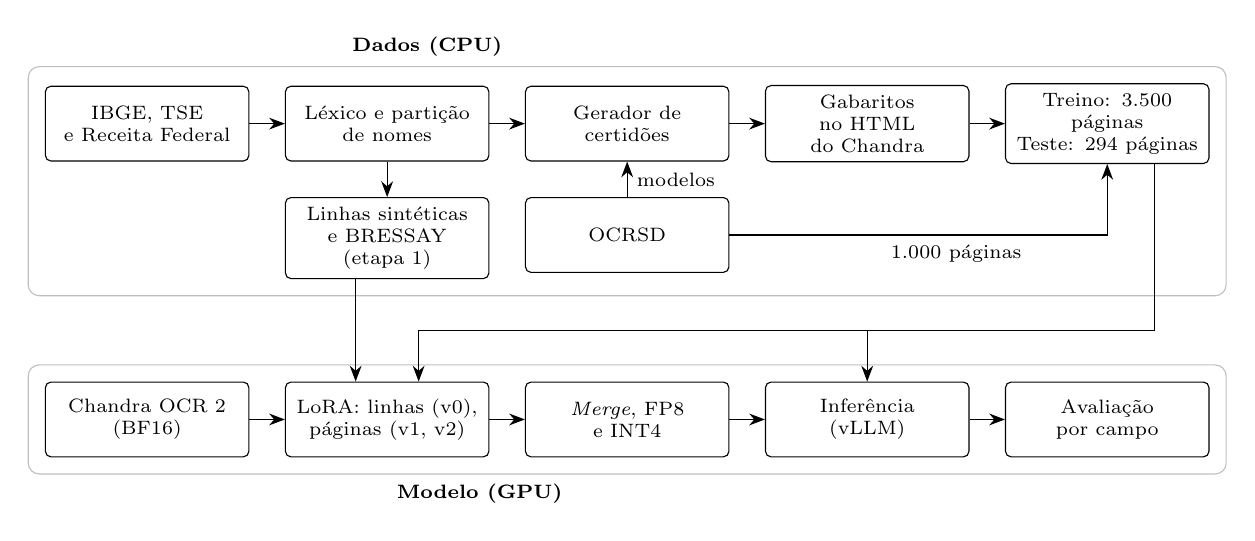
\begin{tikzpicture}[
    font=\scriptsize,
    box/.style={draw, rounded corners=2pt, align=center, minimum height=0.95cm, text width=2.35cm, fill=white},
    arr/.style={-{Stealth[length=2mm]}},
    lane/.style={draw=gray!50, rounded corners=4pt, inner sep=6pt}]
  % dados
  \node[box] (fontes) {IBGE, TSE\\e Receita Federal};
  \node[box, right=0.45cm of fontes] (lexico) {Léxico e partição\\de nomes};
  \node[box, right=0.45cm of lexico] (gerador) {Gerador de\\certidões};
  \node[box, right=0.45cm of gerador] (alvos) {Gabaritos no HTML\\do Chandra};
  \node[box, right=0.45cm of alvos] (conj) {Treino: 3.500 páginas\\Teste: 294 páginas};
  \node[box, below=0.45cm of lexico] (linhas) {Linhas sintéticas\\e BRESSAY (etapa 1)};
  \node[box, below=0.45cm of gerador] (ocrsd) {OCRSD};
  \draw[arr] (fontes) -- (lexico);
  \draw[arr] (lexico) -- (gerador);
  \draw[arr] (gerador) -- (alvos);
  \draw[arr] (alvos) -- (conj);
  \draw[arr] (lexico) -- (linhas);
  \draw[arr] (ocrsd) -- node[right] {modelos} (gerador);
  \draw[arr] (ocrsd.east) -| node[pos=0.3, below] {1.000 páginas} (conj.south);
  \begin{scope}[on background layer]
    \node[lane, fit=(fontes)(conj)(linhas)(ocrsd), label={[font=\scriptsize\bfseries]above left:Dados (CPU)}] (l1) {};
  \end{scope}
  % modelo
  \node[box, below=1.3cm of linhas.south -| fontes] (chandra) {Chandra OCR 2\\(BF16)};
  \node[box, right=0.45cm of chandra] (lora) {LoRA: linhas (v0),\\páginas (v1, v2)};
  \node[box, right=0.45cm of lora] (quant) {\emph{Merge}, FP8\\e INT4};
  \node[box, right=0.45cm of quant] (vllm) {Inferência\\(vLLM)};
  \node[box, right=0.45cm of vllm] (aval) {Avaliação\\por campo};
  \draw[arr] (chandra) -- (lora);
  \draw[arr] (lora) -- (quant);
  \draw[arr] (quant) -- (vllm);
  \draw[arr] (vllm) -- (aval);
  \begin{scope}[on background layer]
    \node[lane, fit=(chandra)(aval), label={[font=\scriptsize\bfseries]below left:Modelo (GPU)}] (l2) {};
  \end{scope}
  \draw[arr] ([xshift=-4mm]linhas.south) -- ([xshift=-4mm]lora.north);
  \coordinate (s) at ($(l1.south)!0.5!(l2.north)$);
  \draw[arr] ([xshift=6mm]conj.south) -- ([xshift=6mm]conj.south |- s) -| ([xshift=4mm]lora.north);
  \draw[arr] ([xshift=6mm]conj.south |- s) -| (vllm.north);
\end{tikzpicture}
\caption{Arquitetura da PoC. O Chandra original é lido com a mesma inferência e avaliado nos mesmos testes, como referência.}
\label{fig:arquitetura}
\end{figure}

% --------------------------------------------------------------
\subsection{Fluxo de Funcionamento}

A parte de linhas roda pelo \texttt{scripts/run.sh}, nas etapas \texttt{lexicon}, \texttt{fonts}, \texttt{bressay}, \texttt{generate}, \texttt{mix}, \texttt{baseline}, \texttt{treino}, \texttt{quantizar} e \texttt{avaliacao}, e cada etapa grava a sua saída em disco e pode ser repetida sem refazer as anteriores. A parte de páginas segue os módulos abaixo, com a configuração de cada treino em \texttt{configs/paginas.yaml} (lora\_v1) e \texttt{configs/paginas\_v2.yaml} (lora\_v2).

\begin{enumerate}
    \item \texttt{scripts/ocrsd/gen.py} e \texttt{extract.py} pedem os lotes ao OCRSD, extraem as páginas e os campos e marcam os campos cuja tinta perdeu os acentos.
    \item \texttt{ocr06.forms.build} gera as certidões locais a partir dos modelos em branco do OCRSD, com nomes do léxico, uma mão por página e um nível de dificuldade.
    \item \texttt{ocr06.forms.targets} monta os gabaritos no HTML do Chandra, com o peso de cada trecho na \emph{loss}.
    \item \texttt{ocr06.model.train} treina o LoRA com a \emph{loss} ponderada e o currículo.
    \item \texttt{ocr06.model.merge} faz o \emph{merge} do adaptador e gera as versões FP8 e INT4.
    \item \texttt{ocr06.model.pages\_infer} e \texttt{ocr06.pages\_eval} transcrevem as páginas de teste com o vLLM e pontuam os campos.
\end{enumerate}

% --------------------------------------------------------------
\subsection{Ferramentas e Tecnologias Utilizadas}

\begin{table}[H]
\centering
\small
\begin{tabular}{@{}p{3.4cm}p{5.2cm}p{6.0cm}@{}}
\toprule
Componente & Escolha & Motivo \\
\midrule
Modelo base & Chandra OCR 2 (BF16) \cite{chandra2026} & Especializado em OCR de página e manuscrito; com cerca de 5 bilhões de parâmetros, cabe em uma GPU sem quantização. \\
GPU & RTX PRO 6000 (96~GB), no Google Colab & Memória para o treino em BF16 com páginas de até 2.048~px. \\
\emph{Fine-tuning} & LoRA com \texttt{transformers} + \texttt{peft} \cite{peft2022} & Suporte ao Qwen3.5 e controle da \emph{loss} por \emph{token}. \\
Inferência & vLLM \cite{vllm2023} & Inferência em lote, com suporte ao Chandra e às versões FP8 e INT4. \\
Quantização & FP8 dinâmico e W4A16 com \texttt{llm-compressor} \cite{llmcompressor} & Não precisam de dados de calibração; o FP8 usa a mesma receita do FP8 público do Chandra \cite{chandrafp8}. \\
Linhas sintéticas & Pillow + OpenCV + Augraphy \cite{augraphy2022} & Renderização com fontes manuscritas e degradação de documento escaneado. \\
Certidões sintéticas & OCRSD \cite{ocrsd} e gerador local & Modelos de documento reais de Registro Civil, com nomes do léxico no gerador local. \\
Escrita neural & VATr++ \cite{vatrpp2024} e Graves \cite{graves2013} & Variação natural da letra dentro e entre escritores. \\
Avaliação de páginas & Python puro (\texttt{pages\_eval.py}) & Campo procurado pela posição, intervalos de confiança pareados e McNemar. \\
Controles de saída & Python puro (\texttt{guard.py}) & Confiança por palavra e sinais de revisão, testáveis em CPU sem o modelo. \\
\bottomrule
\end{tabular}
\caption{Componentes selecionados.}
\end{table}

% --------------------------------------------------------------
\subsection{Definição e Preparação dos Dados}
\label{subsec:dados}

\subsubsection{Fontes de nomes}
A lista completa de prenomes do Censo 2010 (100.787 nomes) veio do espelho do Brasil.IO \cite{brasilio_nomes}, conferido contra o ranking da API oficial do IBGE \cite{ibge_nomes}, e dela foram descartadas 276 grafias que parecem erro de digitação do censo, como ``MMARIA''. Os sobrenomes foram contados em 823.956 candidatos do TSE \cite{tse_eleitorado} e 3.244.525 sócios pessoa física da Receita \cite{rfb_socios}, sem guardar os nomes completos, e ficaram 60.627 com pelo menos 5 ocorrências. Das mesmas fontes saem a distribuição do número de sobrenomes (61\% das pessoas têm dois), a frequência de prenome composto (37\%), as partículas de cada sobrenome (``da Silva'', ``dos Santos'') e as grafias com e sem acento. Os 5.570 municípios vêm da API do IBGE, com a população do Censo 2022.

\subsubsection{Seleção do vocabulário e partição}
Os nomes entram no vocabulário por ordem de frequência na população, até a maior lista em que cada nome aparece, em valor esperado, pelo menos duas vezes no número de imagens configurado. Dentro do vocabulário, o sorteio usa uma temperatura,
\[
q_i = \frac{p_i^{\alpha}}{\sum_j p_j^{\alpha}}, \qquad \alpha = 0{,}5,
\]
para que os nomes mais comuns não dominem o treino. Os nomes que somam os primeiros 80\% da população são os comuns e aparecem em treino, validação e teste, e entre os demais (raros) 10\% ficam reservados ao teste e 5\% à validação. A mesma partição vale para as linhas e para as certidões geradas.

\subsubsection{Linhas}
\label{subsec:dados-linhas}
Cada linha sintética segue um de oito modelos de texto de registro (``Nome: ...'', ``filho de ... e de ...'', ``natural de Cidade - UF'') e é escrita com uma de 85 fontes manuscritas do Google Fonts com os acentos do português, 17 delas reservadas ao teste. A inclinação, a espessura e a linha de base são sorteadas por linha, cada letra é deformada à parte e o Augraphy aplica a degradação de documento escaneado (exemplos na Figura~\ref{fig:exemplos-v2}, no Apêndice~\ref{app:linhas}).

O BRESSAY tem 1.000 redações, cada uma de um autor, com 30.090 linhas transcritas e partição oficial por autor \cite{bressay2023}, e sem as linhas com trecho ilegível ou riscado ficaram 26.135. O treino de linhas teve 40.000 linhas sintéticas e 16.915 do BRESSAY (29,7\% de dados reais), e os testes foram 4.000 linhas sintéticas, com 13.672 nomes, 8.508 deles ausentes do treino, e 5.146 linhas do BRESSAY de autores fora do treino. Metade das conversas de treino usa um \emph{prompt} curto (``Transcreva exatamente o texto manuscrito desta imagem [...] Não corrija nomes.'') e metade o \emph{prompt} nativo do Chandra, que pede o HTML da página.

\subsubsection{Páginas}
\label{subsec:dados-paginas}
As certidões vêm do OCRSD e de um gerador local, nos cinco documentos de Registro Civil que o OCRSD gera com todos os campos preenchidos (certidão de casamento nos modelos antigo e CNJ, certidão de nascimento CNJ, certidão de óbito e Declaração de Nascido Vivo, a DNV).

Do OCRSD foram extraídas 1.000 páginas (240 de casamento antigo, 230 de casamento CNJ, 200 de nascimento, 200 de óbito e 130 DNV), escritas por fontes ou por escritores neurais. Como os escritores neurais não desenham acentos, cada campo guarda o valor pedido e o valor desenhado, e os campos que perderam acentos ficam fora da \emph{loss} e da avaliação. Os registros do OCRSD usam poucos nomes, todos comuns, e essas páginas servem para caligrafia e layout, enquanto os nomes raros vêm do gerador local.

O gerador local usa os modelos em branco e os mapas de campos do OCRSD. Para cada página, ele sorteia um registro do OCRSD e troca cada prenome, sobrenome e município dele, na página inteira, por um sorteado do léxico, dentro da partição. Cada página tem uma mão e uma caneta, com o VATr++ em cerca de metade das páginas de treino, fontes manuscritas em 29\% (29 fontes no treino e 2 reservadas ao teste) e o Graves em 20\%. Os geradores neurais só escrevem texto sem acento, e nas páginas escritas por eles os campos com acento ficam em branco, tanto na imagem quanto no gabarito. Cada página recebe um de quatro níveis de dificuldade, com letras deformadas e fundidas, falhas e borrões de tinta, papel com sombra, ruído e compressão JPEG, e é gravada com lado maior de 2.048~px (Figura~\ref{fig:gerador}).

\begin{figure}[H]
\centering
\begin{subfigure}{0.31\textwidth}
\centering
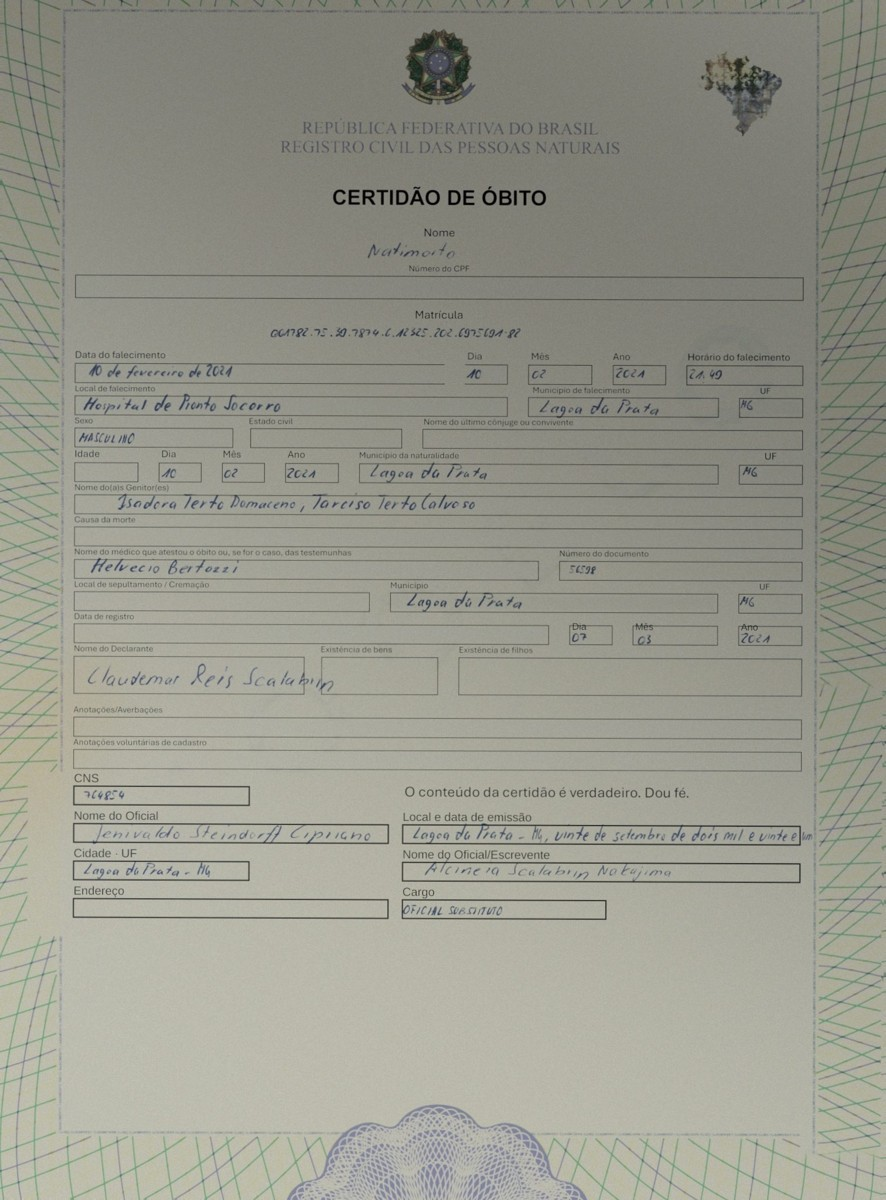
\includegraphics[width=\linewidth]{figuras/gerador_pagina.jpg}
\caption{Página inteira.}
\end{subfigure}
\hfill
\begin{subfigure}{0.66\textwidth}
\centering
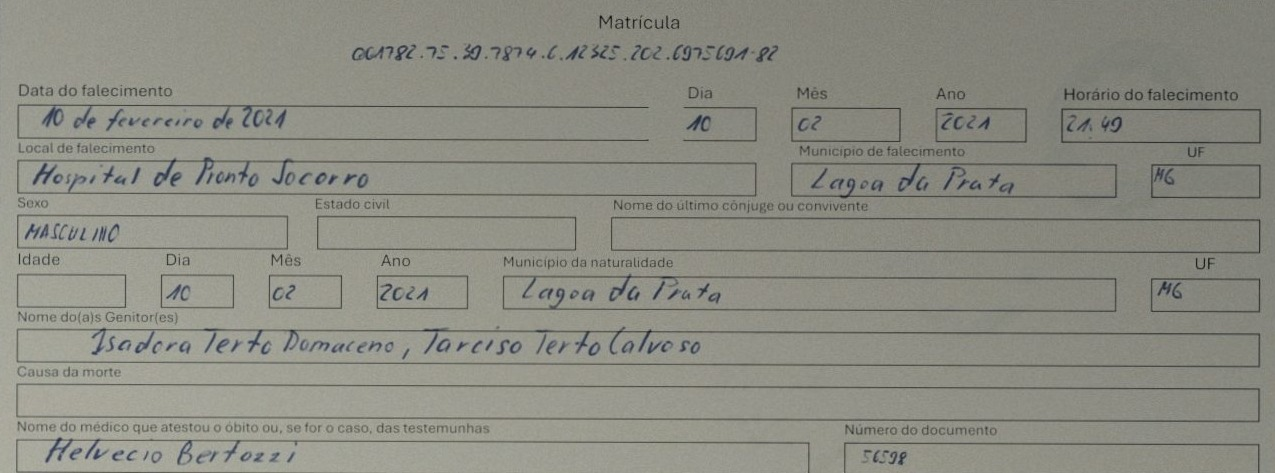
\includegraphics[width=\linewidth]{figuras/gerador_zoom_1.jpg}
\caption{Ampliação, da matrícula aos genitores.}
\end{subfigure}
\caption{Certidão de óbito do teste difícil, escrita pelo VATr++ no nível 2. Os nomes e o município são do léxico. Os campos vazios, como cônjuge e idade, também estão vazios no registro do OCRSD, que é de um natimorto.}
\label{fig:gerador}
\end{figure}

No gabarito de cada página, o texto impresso foi tirado da saída do próprio Chandra no modelo em branco, e os valores manuscritos entram nos blocos de cada campo, no mesmo HTML que o modelo já devolve. Na \emph{loss}, o texto impresso tem peso 0,3, os valores manuscritos peso 1 e os campos que perderam acento peso 0, e no lora\_v2 os nomes têm peso 2.

O teste difícil (Tabela~\ref{tab:conjuntos-paginas}) foi montado para medir nomes inéditos, com 70\% das palavras de nome tiradas da parte reservada ao teste, as duas fontes reservadas e estilos de escritor neural que não aparecem no treino. Só 17 dos seus 440 campos de nome têm todas as palavras presentes em alguma página de treino. O teste normal usa nomes sorteados pela frequência real, como num cartório. Nenhuma página dos testes aparece no treino (conferido pelo identificador e pela imagem).

\begin{table}[H]
\centering
\small
\begin{tabular}{@{}lrrp{7.2cm}@{}}
\toprule
Conjunto & Locais & OCRSD & Uso \\
\midrule
Treino do lora\_v1 & 941 & 859 & Treino a partir do Chandra original \\
Treino do lora\_v2 & 1.559 & 141 & Continuação do lora\_v1, com nomes de peso 2 \\
Teste difícil & 100 & -- & 2.648 campos, 440 de nome; nomes, fontes e escritores reservados \\
Teste normal & 100 & -- & 2.668 campos, 488 de nome; nomes pela frequência real \\
Teste do OCRSD & -- & 94 & 1.460 campos, 399 de nome; 47 páginas com fontes do treino e 47 com estilos neurais reservados (só lora\_v1) \\
\bottomrule
\end{tabular}
\caption{Conjuntos de páginas. As 141 páginas do OCRSD do treino do lora\_v2 incluem as 94 do teste do OCRSD, que foram usadas para avaliar o lora\_v1 antes de entrarem no treino.}
\label{tab:conjuntos-paginas}
\end{table}

% --------------------------------------------------------------
\subsection{Fine-tuning}
\label{subsec:ajuste}

Nas duas etapas, o LoRA tem \emph{rank} 16, $\alpha_{\text{LoRA}} = 32$ e \emph{dropout} de 0,05 em todas as camadas lineares do modelo de linguagem, inclusive as de atenção linear, com o encoder de visão congelado (32,5 milhões de parâmetros treináveis, 0,71\% do modelo). Os hiperparâmetros foram fixados antes de qualquer teste e não foram mudados depois.

Em linhas, o lora\_v0 treinou por uma época, 3.558 passos com \emph{batch} de 16 linhas, \emph{learning rate} de $10^{-4}$, \emph{warmup} de 3\% e decaimento cosseno, em 3,1~horas. O \emph{checkpoint} foi escolhido pela \emph{loss} de validação do BRESSAY, separada da do sintético, para que decorar as fontes sintéticas não escondesse uma piora na caligrafia real.

Em páginas, cada exemplo é uma página inteira com lado maior de 2.048~px, cerca de 5,9 mil \emph{tokens} numa página do OCRSD. O treino usa \emph{batch} efetivo de 16 páginas, \emph{learning rate} constante de $10^{-4}$ depois de 3\% de \emph{warmup} e uma época, com as páginas ordenadas do nível 1 ao 4 (\emph{curriculum learning}). A \emph{loss} é a entropia cruzada ponderada pelos pesos do gabarito,
\[
\mathcal{L} = \frac{\sum_t w_t\, \ell_t}{\sum_t w_t}, \qquad
w_t^{\text{nome}} = 2\,\bigl(1 + \beta\,(1 - p_t)\bigr),
\]
em que $\ell_t$ é a entropia cruzada do \emph{token} $t$. No lora\_v2, os \emph{tokens} de nome recebem um peso que cresce com a probabilidade $1 - p_t$ que o modelo deixou de dar ao \emph{token} certo, com $\beta = 2$ e sem gradiente pelo fator. Um nome lido com confiança pesa 2, e um nome errado pesa até 6. O lora\_v1 partiu do Chandra original e treinou 113 passos em 66~min, e o lora\_v2 continuou o lora\_v1 por 107 passos em 65~min, com pico de 60,7~GB na GPU. A validação usa 40 páginas fixas do próprio treino e serviu só para escolher o \emph{checkpoint}.

Depois do treino, o adaptador passa por \emph{merge} com o modelo em BF16, e o modelo resultante é quantizado em FP8 dinâmico e em W4A16 (INT4). A quantização vale para as camadas lineares de atenção completa e para as MLPs do modelo de linguagem, e o encoder de visão, as camadas de atenção linear, os \emph{embeddings} e a camada de saída continuam em BF16. A mesma receita FP8 foi aplicada ao Chandra original, para comparação.

% --------------------------------------------------------------
\subsection{Estratégia de Avaliação}
\label{subsec:aval}

Em linhas, a avaliação usa o teste sintético, com nomes e fontes reservados, e o do BRESSAY, com autores fora do treino. O CER e o WER somam a distância de Levenshtein sobre o conjunto, e a predição é alinhada ao gabarito por palavra, para separar o erro por tipo de nome, por grupo de frequência e entre nomes vistos e inéditos. No \emph{prompt} nativo, o HTML é removido antes da medição.

Nas certidões, todos os modelos leem as mesmas páginas com o \emph{prompt} nativo, a mesma resolução, \emph{greedy decoding} e no máximo 6.144 \emph{tokens} de saída. Cada campo manuscrito do gabarito tem uma caixa, e a leitura do modelo é o trecho mais parecido com o valor certo dentro dos blocos da saída cuja caixa encosta na do campo. O campo está certo quando esse trecho é idêntico ao valor (acerto exato local). Campos numéricos são comparados só por letras e dígitos, campos de até 3 caracteres são contados à parte e campos que perderam acentos ficam de fora. Por página, mede-se a completude (fração dos campos encontrados com CER de até 20\% em qualquer ponto da saída), o truncamento e o \emph{loop} (trecho repetido três vezes ou mais, ou saída 50\% maior que a dos outros modelos). As diferenças entre modelos são calculadas nas mesmas páginas, com intervalo de confiança de 95\% por \emph{bootstrap} pareado sobre as páginas (1.000 reamostragens) e teste de McNemar campo a campo. As métricas, os testes e as regras de decisão foram fixados antes da primeira execução dos modelos treinados.

Fora das certidões, a avaliação usa as 199 páginas de teste do BRESSAY, com o CER do texto da página, e os 50 formulários reais de validação do XFUND-PT \cite{xfund2022}. Nos formulários, os campos preenchidos foram apagados e reescritos com as fontes reservadas ao teste, e cada um é procurado em qualquer ponto da saída.

% --------------------------------------------------------------
\subsection{Critérios de Aceitação da PoC}

\begin{enumerate}
    \item Partições sem vazamento, sem nome reservado ao teste no treino, sem autor do BRESSAY em mais de um conjunto e sem página de teste no treino. Atendido (Experimento 1 e Seção~\ref{subsec:dados-paginas}).
    \item Treino completo em uma única GPU. Atendido, com pico de 49,5~GB em linhas e 60,7~GB em páginas.
    \item Acerto em nomes maior que o do modelo original, sem aumento de truncamento ou \emph{loop}. Atendido em linhas (nomes inéditos de 70,9\% para 79,7\%) e nas certidões, com intervalo de confiança acima de zero (nomes de 24,3\% para 32,5\% e de 40,4\% para 50,2\%, sem nenhuma página truncada ou em \emph{loop}).
    \item Sem piora fora do domínio do treino. Atendido pelo lora\_v0, que reduziu o CER das páginas do BRESSAY de 26,5\% para 17,3\%, e não atendido pelo lora\_v2, que o elevou para 48,6\% (Experimento 7).
    \item Erro em nomes inéditos próximo do erro em nomes vistos e nenhum nome do treino extraído. A primeira parte foi atendida em linhas e no teste normal de páginas, e os testes de extração não foram executados.
    \item Versão quantizada com perda de até 1 ponto em nomes exatos e sem aumento de truncamento ou \emph{loop}. O FP8 atende no teste normal ($-0{,}6$ ponto) e fica 1,8 ponto abaixo no difícil, e o INT4 atende no normal ($-0{,}8$) e perde 3,6 pontos no difícil. Nenhuma versão quantizada teve página truncada ou em \emph{loop}.
\end{enumerate}

% ==============================================================
% SEÇÃO 7 — AVALIAÇÃO EXPERIMENTAL (*)
% ==============================================================
\section{Avaliação Experimental}
\label{sec:avaliacao}

% --------------------------------------------------------------
\subsection{Experimento 1: Validação sem o Modelo}
\label{subsec:exp1}

Com 40 mil imagens de treino, o vocabulário fica com cerca de 10 mil prenomes, 19 mil sobrenomes e 3,8 mil municípios (de 94\% a 97\% da população), e com $\alpha = 0{,}5$ os 10 prenomes mais comuns caem de 21,1\% para 2,3\% dos sorteios. Nenhum dos 2.909 nomes reservados ao teste apareceu nas 20 mil linhas de treino verificadas, e a geração das linhas (40 mil de treino, 2 mil de validação e 4 mil de teste) levou 12,5 minutos em 16 núcleos de CPU. No BRESSAY só 38 nomes do teste são inéditos, e ele mede sobretudo a leitura de caligrafia real. A evidência sobre nomes inéditos vem dos testes sintéticos.

A avaliação foi testada com predições montadas a partir do próprio gabarito, com erros inseridos de forma controlada. Em linhas, o CER medido coincidiu com o esperado nos 14 casos (sete tipos de erro em dois testes). O alinhamento dos nomes é feito por palavra porque, por caractere, um nome omitido era associado a letras das palavras vizinhas (CER de 97\% em vez de 100\%). O \texttt{guard.py} não marcou nenhum dos 9.146 gabaritos de teste e deixou passar 78 de 915 saídas defeituosas montadas a partir deles, todas do tipo longa demais. O avaliador de páginas e o modo de página do treino têm 21 testes automatizados, que rodam em CPU sem os pesos do Chandra.

% --------------------------------------------------------------
\subsection{Experimento 2: Treino em Linhas}
\label{subsec:exp2}

A \emph{loss} de validação do lora\_v0 caiu em todas as avaliações, de 0,457 para 0,341 no BRESSAY e de 0,363 para 0,291 no sintético, e o melhor \emph{checkpoint} foi o último.

\begin{table}[H]
\centering
\small
\begin{tabular}{@{}lrrrr@{}}
\toprule
& \multicolumn{2}{c}{BRESSAY (5.146 linhas)} & \multicolumn{2}{c}{Sintético (4.000 linhas)} \\
(\%) & Chandra & lora\_v0 & Chandra & lora\_v0 \\
\midrule
CER & 20,1 & \textbf{4,9} & 8,6 & \textbf{3,4} \\
Linhas sem erro & 12,6 & \textbf{33,5} & 47,2 & \textbf{65,5} \\
Nomes sem erro & 66,4 & \textbf{79,0} & 74,6 & \textbf{83,6} \\
Nomes inéditos sem erro & -- & -- & 70,9 & \textbf{79,7} \\
\bottomrule
\end{tabular}
\caption{Resultados em linhas, com o \emph{prompt} nativo do Chandra. O teste sintético tem 17 fontes e 8.508 nomes fora do treino; o BRESSAY tem só 38 nomes inéditos, poucos para a última linha. A tabela completa, com o \emph{prompt} curto e as versões FP8, está no Apêndice~\ref{app:linhas}.}
\label{tab:linhas}
\end{table}

No BRESSAY, o CER caiu de 20,1\% para 4,9\%, e as linhas sem nenhum erro passaram de uma em cada oito para uma em cada três (Tabela~\ref{tab:linhas}). O Chandra original completa palavras cortadas no fim da linha, troca palavras por outras mais prováveis, às vezes muda de idioma (``distúrbios psíquicos'' lido como ``distúrbien pequeños de los niños'') e entrou em \emph{loop} em 76 linhas, contra nenhuma do lora\_v0.

No teste sintético, com fontes e nomes fora do treino, os nomes inéditos lidos sem erro subiram de 70,9\% para 79,7\%. O CER dos nomes vistos e dos inéditos caiu junto (de 7,1\% e 9,4\% para 3,4\% e 5,5\%), e a diferença entre eles foi de 2,3 para 2,1 pontos, quando decorar os nomes do treino a teria aumentado. Ainda sobram nomes raros trocados pela forma comum, como ``Zamprogna'' lido como ``Zampogna''. A versão FP8 do lora\_v0 ficou a no máximo 0,1 ponto de CER da BF16 e leu de 16\% a 21\% mais linhas por segundo no vLLM. Depois do treino, o \emph{prompt} curto e o nativo passaram a dar praticamente o mesmo resultado.

Com o \emph{prompt} curto, o \texttt{guard.py} mandou para revisão 56,9\% das linhas do BRESSAY lidas pelo lora\_v0, com CER de 7,6\% nas marcadas e 1,0\% nas aprovadas, e 27,8\% das sintéticas, com 8,7\% e 0,7\% (Tabela~\ref{tab:guard}). Cerca de um quarto das linhas erradas (24,5\% no BRESSAY e 31,6\% no sintético) passou sem marcação, com confiança alta.

% --------------------------------------------------------------
\subsection{Experimento 3: Linhas e Páginas nas Mesmas Certidões}
\label{subsec:linhas-paginas}

Aplicado a 38 certidões do teste difícil, o lora\_v0 leu 1,2 ponto a menos que o Chandra nos campos e 2,8 pontos a mais nos nomes (Tabela~\ref{tab:linhas-paginas}), e em 47 páginas do OCRSD lidas na mesma ocasião o acerto ficou igual (84,7\% e 84,4\%). Nas mesmas 38 certidões, o lora\_v1 e o lora\_v2, treinados com páginas inteiras, leram 70,8\% e 73,2\% dos campos. O adaptador de linhas só tinha visto recortes de uma linha, sem os rótulos impressos, as caixas e a ordem de leitura de um formulário. No BRESSAY, que é o domínio do treino dele, ele reduziu o CER de página de 26,5\% para 17,3\% (Experimento 7).

\begin{table}[H]
\centering
\small
\begin{tabular}{@{}lrrrr@{}}
\toprule
Mesmas 38 certidões do teste difícil (\%) & Chandra & lora\_v0 & lora\_v1 & lora\_v2 \\
\midrule
Campos manuscritos sem erro (1.068) & 56,6 & 55,4 & 70,8 & \textbf{73,2} \\
Nomes sem erro (176) & 19,9 & 22,7 & 25,6 & \textbf{27,8} \\
\bottomrule
\end{tabular}
\caption{Adaptadores das duas etapas nas mesmas certidões. O Chandra e o lora\_v0 vêm da execução da primeira etapa; na execução da segunda, a mesma do lora\_v1 e do lora\_v2, o Chandra acertou 58,0\% dos campos e 19,9\% dos nomes nessas páginas.}
\label{tab:linhas-paginas}
\end{table}

% --------------------------------------------------------------
\subsection{Experimento 4: Treino em Páginas Inteiras}
\label{subsec:exp4}

\subsubsection{Testes difícil e normal}
O lora\_v2 leu sem erro 72,2\% e 72,0\% dos campos manuscritos nos testes difícil e normal, contra 55,4\% e 55,8\% do Chandra, e 32,5\% e 50,2\% dos nomes, contra 24,3\% e 40,4\% (Tabela~\ref{tab:paginas}), todas as diferenças com intervalo de confiança acima de zero. Em campos, o lora\_v2 acertou 500 que o Chandra errava e errou 54 que ele acertava no teste difícil, e 505 contra 73 no normal. A continuação do treino (lora\_v2 sobre o lora\_v1) somou 2,4 e 2,9 pontos nos campos, ambos significativos, e 5,7 pontos nos nomes do teste normal, e no teste difícil os nomes subiram 2,0 pontos, com intervalo de $-1{,}9$ a $+6{,}8$.

\begin{table}[H]
\centering
\small
\begin{tabular}{@{}lrrrrrr@{}}
\toprule
& \multicolumn{3}{c}{Teste difícil} & \multicolumn{3}{c}{Teste normal} \\
& Chandra & lora\_v1 & lora\_v2 & Chandra & lora\_v1 & lora\_v2 \\
\midrule
Campos exatos (\%) & 55,4 & 69,8 & \textbf{72,2} & 55,8 & 69,2 & \textbf{72,0} \\
Nomes exatos (\%) & 24,3 & 30,5 & \textbf{32,5} & 40,4 & 44,5 & \textbf{50,2} \\
Completude (\%) & 84,6 & 92,6 & \textbf{93,5} & 85,0 & 92,8 & \textbf{93,1} \\
Páginas truncadas & 1 & 0 & 0 & 6 & 0 & 0 \\
Páginas em \emph{loop} & 1 & 0 & 0 & 3 & 0 & 0 \\
\midrule
\multicolumn{7}{@{}l}{\textit{Diferença lora\_v2 $-$ Chandra, em pontos (IC 95\%)}} \\
Campos & \multicolumn{3}{c}{+16,8 (+14,6 a +19,3)} & \multicolumn{3}{c}{+16,2 (+13,9 a +18,6)} \\
Nomes & \multicolumn{3}{c}{+8,2 (+3,8 a +12,6)} & \multicolumn{3}{c}{+9,8 (+5,5 a +14,7)} \\
\multicolumn{7}{@{}l}{\textit{Diferença lora\_v2 $-$ lora\_v1, em pontos (IC 95\%)}} \\
Campos & \multicolumn{3}{c}{+2,4 (+0,6 a +4,1)} & \multicolumn{3}{c}{+2,9 (+1,2 a +4,5)} \\
Nomes & \multicolumn{3}{c}{+2,0 ($-$1,9 a +6,8)} & \multicolumn{3}{c}{+5,7 (+2,1 a +10,0)} \\
\bottomrule
\end{tabular}
\caption{Resultados nos testes de páginas (100 páginas cada; 2.648 e 2.668 campos, 440 e 488 de nome). O lora\_v1 leu o teste difícil numa GPU L4; os demais modelos rodaram na RTX PRO 6000, com a mesma configuração de inferência.}
\label{tab:paginas}
\end{table}

Todas as classes de campo melhoraram (Figura~\ref{fig:classes}), mais nos números, como matrículas, CPFs e números de documento (de 59,8\% para 86,7\% no teste difícil), e no texto livre, como endereços e filiação por extenso (de 42,8\% para 61,9\%). As datas foram de 75,2\% para 91,7\%. Os nomes continuam com o menor acerto, porque cada campo tem várias palavras raras.

\begin{figure}[H]
\centering
\begin{subfigure}{\textwidth}
\centering
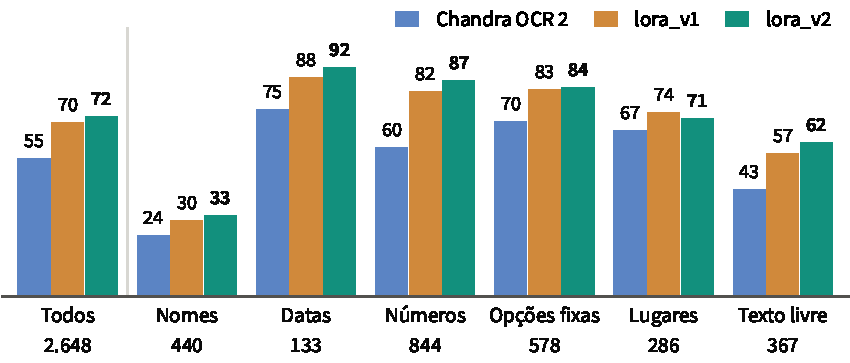
\includegraphics[width=0.92\textwidth]{figuras/g_dificil.pdf}
\caption{Teste difícil.}
\end{subfigure}

\vspace{2mm}
\begin{subfigure}{\textwidth}
\centering
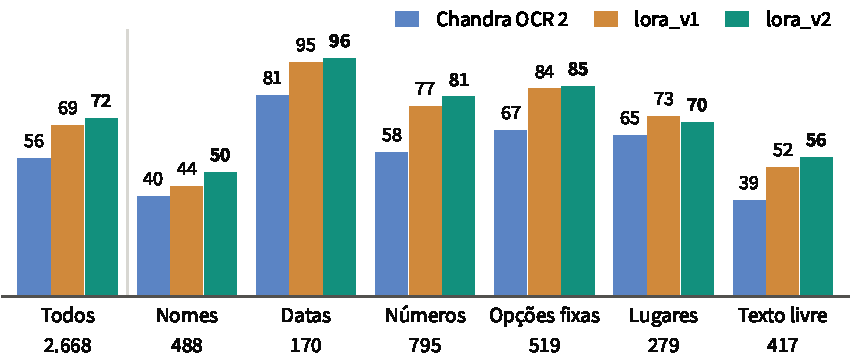
\includegraphics[width=0.92\textwidth]{figuras/g_normal.pdf}
\caption{Teste normal.}
\end{subfigure}
\caption{Acerto exato (\%) por classe de campo. Abaixo de cada classe, o número de campos.}
\label{fig:classes}
\end{figure}

O mesmo adaptador, treinado com os cinco documentos juntos, melhorou todos eles, de 11 a 21 pontos nos campos (Tabela~\ref{tab:templates}), e com 13 a 35 páginas por documento não é possível dizer quais ganharam mais.

\begin{table}[H]
\centering
\small
\begin{tabular}{@{}lrrrrrr@{}}
\toprule
& \multicolumn{3}{c}{Teste difícil} & \multicolumn{3}{c}{Teste normal} \\
Documento & Páginas & Chandra & lora\_v2 & Páginas & Chandra & lora\_v2 \\
\midrule
Casamento (modelo antigo) & 16 & 48,4 & 62,6 & 13 & 50,6 & 71,4 \\
Casamento (CNJ) & 17 & 49,5 & 66,8 & 23 & 55,1 & 70,7 \\
Nascimento (CNJ) & 16 & 49,0 & 60,7 & 16 & 52,8 & 65,1 \\
Óbito & 16 & 54,0 & 68,9 & 22 & 59,8 & 71,0 \\
DNV & 35 & 59,9 & 78,7 & 26 & 55,7 & 76,0 \\
\bottomrule
\end{tabular}
\caption{Campos manuscritos sem erro (\%) por documento.}
\label{tab:templates}
\end{table}

Numa certidão de óbito do teste difícil (Figura~\ref{fig:demo}), da matrícula para baixo, o Chandra acertou 17 dos 21 campos manuscritos e o lora\_v2, 20. O Chandra errou a matrícula, o horário (``21:49'' lido como ``21.49''), um sobrenome dos genitores e o prenome do declarante (``Claudemar'' lido como ``Claudemir''), e o lora\_v2 errou o prenome raro do campo do escrevente (``Alcineia'' lido como ``Alineia'').

\begin{figure}[H]
\centering
\begin{subfigure}{0.49\textwidth}
\centering
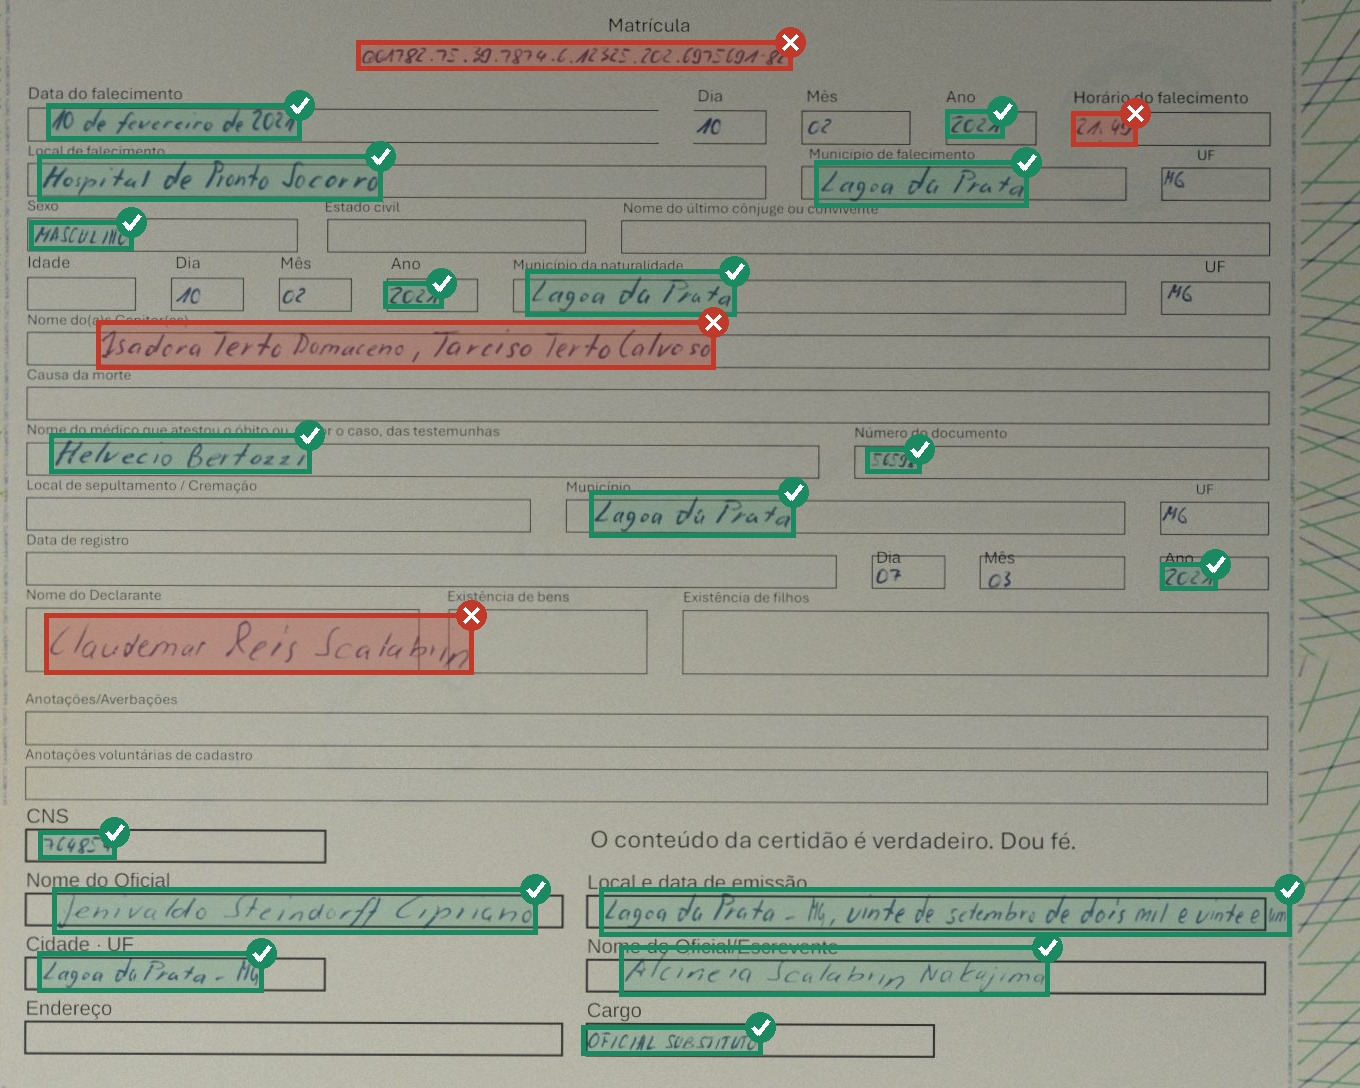
\includegraphics[width=\linewidth]{figuras/certidao_original.jpg}
\caption{Chandra OCR 2: 17 de 21 campos.}
\end{subfigure}
\hfill
\begin{subfigure}{0.49\textwidth}
\centering
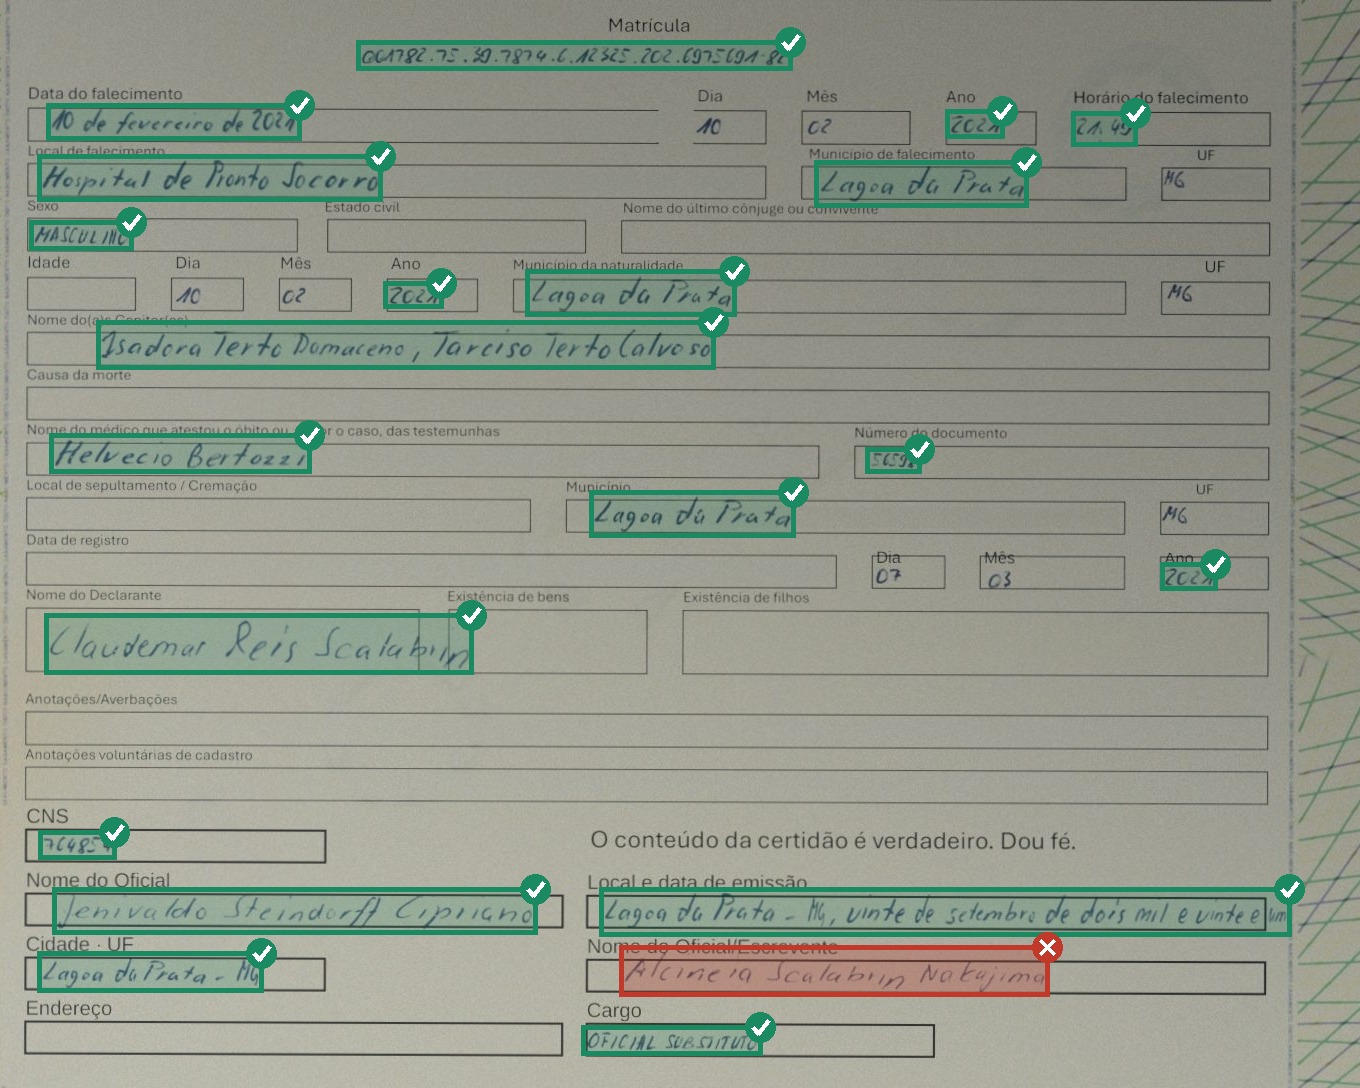
\includegraphics[width=\linewidth]{figuras/certidao_ajustado.jpg}
\caption{lora\_v2: 20 de 21 campos.}
\end{subfigure}
\caption{A mesma certidão do teste difícil, escrita pelo VATr++, com os campos manuscritos lidos sem erro em verde e os errados em vermelho.}
\label{fig:demo}
\end{figure}

Dos 500 campos do teste difícil que o lora\_v2 corrigiu, a leitura do Chandra estava a um caractere do valor certo em 228 (46\%) e a dois em 102 (20\%), como nos exemplos da Tabela~\ref{tab:corrigidos}.

\begin{table}[H]
\centering
\small
\renewcommand{\arraystretch}{1.2}
\begin{tabular}{@{}m{5.6cm}>{\raggedright\arraybackslash}m{4.5cm}>{\raggedright\arraybackslash}m{4.5cm}@{}}
\toprule
Imagem & Chandra & lora\_v2 \\
\midrule
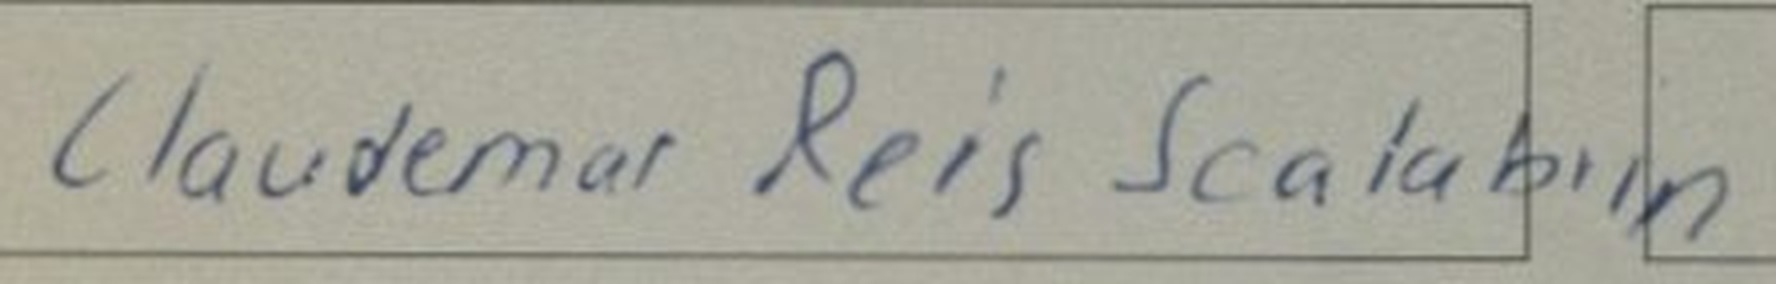
\includegraphics[width=5.4cm,height=9mm,keepaspectratio]{figuras/ex_claudemar.jpg} & Claudemir Reis Scalabrin & Claudemar Reis Scalabrin \\
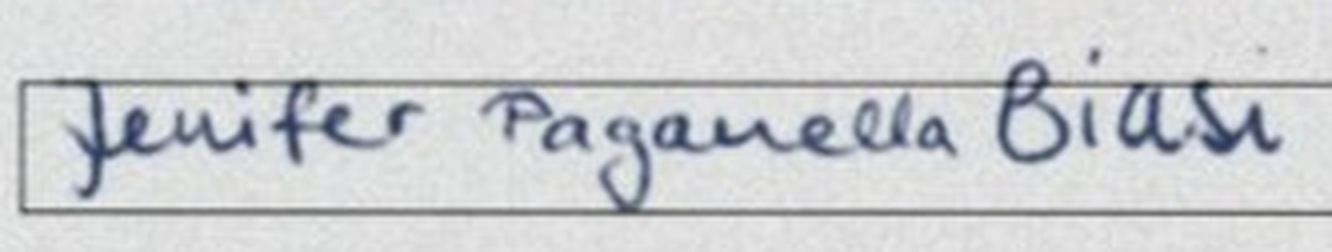
\includegraphics[width=5.4cm,height=9mm,keepaspectratio]{figuras/ex_jenifer.jpg} & Jenifer Paganella Biassi & Jenifer Paganella Biasi \\
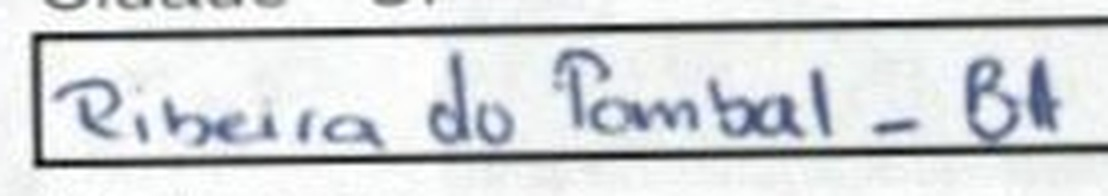
\includegraphics[width=5.4cm,height=9mm,keepaspectratio]{figuras/ex_ribeira.jpg} & Ribeira do Tombal - BA & Ribeira do Pombal - BA \\
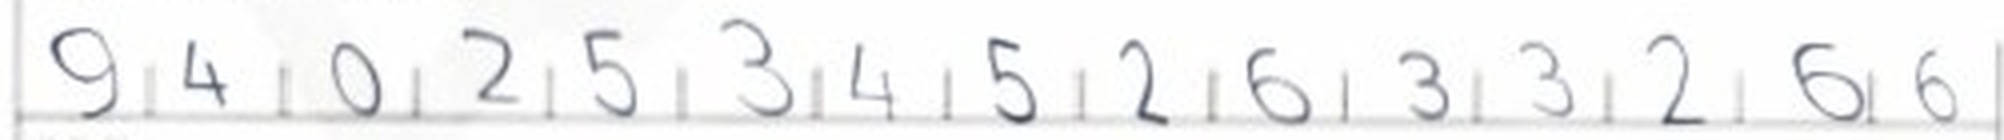
\includegraphics[width=5.4cm,height=9mm,keepaspectratio]{figuras/ex_sus.jpg} & 910253452633266 & 940253452633266 \\
\bottomrule
\end{tabular}
\caption{Campos do teste difícil que o Chandra errou e o lora\_v2 leu sem erro, com a leitura de cada modelo na região do campo. O último é o número do Cartão SUS de uma DNV.}
\label{tab:corrigidos}
\end{table}

Dos 297 campos de nome que o lora\_v2 ainda erra no teste difícil, 125 (42\%) têm o primeiro prenome certo e o erro num sobrenome ou no segundo prenome, e em 68 (23\%) o prenome virou algo fora da lista de prenomes do IBGE, como ``Alineia''. A troca de um prenome raro por um prenome comum, como ``Maikon'' lido como ``Marcia'' e ``Guiomar'' como ``Giovana'' (Tabela~\ref{tab:erros}), aparece em 37 campos (12\%), e outros 39 trocam um prenome raro por outro raro. No teste normal, com menos nomes raros, essa troca aparece em 3 dos 243 campos errados. Em alguns campos o lora\_v2 errou o que o Chandra lia certo, como ``Alcineia''.

\begin{table}[H]
\centering
\small
\renewcommand{\arraystretch}{1.2}
\begin{tabular}{@{}>{\raggedright\arraybackslash}p{4.9cm}>{\raggedright\arraybackslash}p{4.9cm}>{\raggedright\arraybackslash}p{4.9cm}@{}}
\toprule
Gabarito & Chandra & lora\_v2 \\
\midrule
\multicolumn{3}{@{}c@{}}{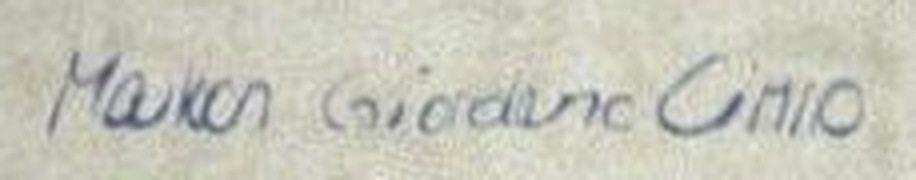
\includegraphics[width=12cm,height=10mm,keepaspectratio]{figuras/ex_maikon.jpg}} \\
Maikon Giordano Cirino & Manoel Giordane Critto & Marcia Giordane Critto \\
\midrule
\multicolumn{3}{@{}c@{}}{
\includegraphics[width=12cm,height=10mm,keepaspectratio]{figuras/ex_guiomar.jpg}} \\
Guiomar Schiavon Arrabal & Geovana Schiaven Ararabal & Giovana Schiaven Araral \\
\midrule
\multicolumn{3}{@{}c@{}}{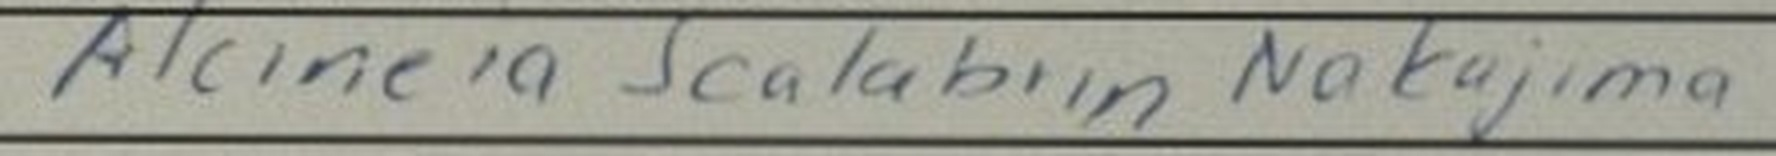
\includegraphics[width=12cm,height=10mm,keepaspectratio]{figuras/ex_alcineia.jpg}} \\
Alcineia Scalabrin Nakajima & Alcineia Scalabrin Nakajima & Alineia Scalabrin Nakajima \\
\bottomrule
\end{tabular}
\caption{Campos de nome do teste difícil que o lora\_v2 ainda erra.}
\label{tab:erros}
\end{table}

Para ver se o ganho em nomes vem de nomes decorados, os campos de nome foram separados entre os que têm todas as palavras presentes em alguma página de treino e os que têm pelo menos uma palavra nunca vista (Tabela~\ref{tab:memo-paginas}). No teste normal, os campos com palavra inédita ganharam 18,2 pontos e os totalmente vistos, 7,1, o contrário do que faria um modelo que decorou os nomes do treino. No teste difícil, quase todos os campos têm palavra inédita (423 de 440) e o acerto neles subiu de 23,9\% para 31,4\%, e os 17 campos totalmente vistos foram de 6 para 10 certos, poucos para concluir qualquer coisa.

\begin{table}[H]
\centering
\small
\begin{tabular}{@{}llrrr@{}}
\toprule
Teste & Campos de nome & Quantidade & Chandra & lora\_v2 \\
\midrule
Difícil & todas as palavras vistas & 17 & 35,3 & 58,8 \\
Difícil & alguma palavra inédita & 423 & 23,9 & 31,4 \\
Normal & todas as palavras vistas & 367 & 44,7 & 51,8 \\
Normal & alguma palavra inédita & 121 & 27,3 & 45,5 \\
\bottomrule
\end{tabular}
\caption{Acerto exato (\%) dos campos de nome, separados pela presença das suas palavras nas 3.500 páginas de treino do lora\_v1 e do lora\_v2.}
\label{tab:memo-paginas}
\end{table}

O texto impresso não tem gabarito independente, já que o do treino veio da saída do próprio Chandra. Contra a saída do Chandra, com os valores manuscritos apagados, o texto impresso do lora\_v2 difere em 26,5\% dos caracteres no teste difícil. A versão FP8 do próprio Chandra, sem nenhum treino, difere da BF16 em 23,2\% na mesma métrica, e a medida é dominada pela divisão em blocos e pela ordem de leitura, sem dizer se o texto impresso piorou.

% --------------------------------------------------------------
\subsection{Experimento 5: Páginas do OCRSD}
\label{subsec:exp5}

O teste do OCRSD tem 94 páginas do mesmo gerador que deu 859 páginas ao treino do lora\_v1, e foi lido pelo lora\_v1 antes de essas páginas entrarem no treino do lora\_v2 (Tabela~\ref{tab:ocrsd}). Metade das páginas usa as duas fontes manuscritas do OCRSD, que também estão no treino, e a outra metade os escritores neurais do OCRSD com estilos que ficaram fora do treino (os mesmos geradores entram no treino com outros estilos). No total, o acerto nos campos foi de 84,6\% para 95,5\% (+10,9 pontos, IC de +8,1 a +14,0), com 172 campos corrigidos e 13 piorados, e a completude de 96,1\% para 99,5\%. Nos 252 campos dos estilos reservados o acerto foi de 77,8\% para 94,0\%, e nos 1.208 escritos com as fontes, de 86,0\% para 95,8\%. Os registros do OCRSD usam 68 prenomes e 35 sobrenomes comuns, e esse teste mede caligrafia e layout, não nomes raros.

\begin{table}[H]
\centering
\small
\begin{tabular}{@{}lrrr@{}}
\toprule
Campos manuscritos & Campos & Chandra & lora\_v1 \\
\midrule
Todos & 1.460 & 84,6 & \textbf{95,5} \\
\quad escritos por estilos neurais fora do treino & 252 & 77,8 & \textbf{94,0} \\
\quad escritos com fontes também usadas no treino & 1.208 & 86,0 & \textbf{95,8} \\
\midrule
Nomes & 399 & 84,7 & \textbf{95,5} \\
Opções fixas (sexo, estado civil) & 244 & 74,6 & \textbf{98,8} \\
Texto livre & 286 & 72,7 & \textbf{91,3} \\
Lugares & 132 & 93,2 & \textbf{98,5} \\
Datas & 94 & 98,9 & 98,9 \\
Números & 305 & \textbf{95,4} & 94,4 \\
\bottomrule
\end{tabular}
\caption{Acerto exato (\%) em 94 páginas do OCRSD, por forma de escrita e por classe de campo.}
\label{tab:ocrsd}
\end{table}

% --------------------------------------------------------------
\subsection{Experimento 6: Quantização e Desempenho}
\label{subsec:exp6}

Contra o lora\_v2 em BF16, o FP8 perdeu 0,5 ponto nos campos do teste difícil (IC de $-1{,}3$ a $+0{,}3$) e 0,1 no normal (Tabela~\ref{tab:quant}). O INT4 perdeu 2,3 pontos nos campos do difícil (IC de $-3{,}4$ a $-1{,}3$) e 3,6 nos nomes (IC de $-7{,}0$ a $-0{,}7$), e no teste normal nenhuma das suas perdas foi significativa ($-0{,}5$ ponto nos campos e $-0{,}8$ nos nomes). A mesma receita FP8 no Chandra original deu 55,1\% nos campos, contra 55,4\% em BF16, e os mesmos 24,3\% nos nomes.

\begin{table}[H]
\centering
\small
\setlength{\tabcolsep}{5pt}
\begin{tabular}{@{}lcc|c|ccc@{}}
\toprule
 & \multicolumn{2}{c|}{Chandra OCR 2} & lora\_v1 & \multicolumn{3}{c}{lora\_v2} \\
 & BF16 & FP8 & BF16 & BF16 & FP8 & INT4 \\
\midrule
\multicolumn{7}{@{}l}{\textit{Teste difícil}} \\
\quad Campos exatos (\%) & 55,4 & 55,1 & 69,8 & \textbf{72,2} & 71,7 & 69,9 \\
\quad Nomes exatos (\%) & 24,3 & 24,3 & 30,5 & \textbf{32,5} & 30,7 & 28,9 \\
\multicolumn{7}{@{}l}{\textit{Teste normal}} \\
\quad Campos exatos (\%) & 55,8 & -- & 69,2 & \textbf{72,0} & 71,9 & 71,6 \\
\quad Nomes exatos (\%) & 40,4 & -- & 44,5 & \textbf{50,2} & 49,6 & 49,4 \\
\multicolumn{7}{@{}l}{\textit{Inferência (RTX PRO 6000, vLLM)}} \\
\quad Pesos na GPU (GiB) & 8,6 & 6,2 & 8,6 & 8,6 & 6,2 & \textbf{5,0} \\
\quad Uma página por vez (s/página) & 23,0 & -- & -- & 22,6 & 17,7 & \textbf{14,9} \\
\quad 48 páginas por vez (s/página) & 1,25 & 1,20 & -- & 1,22 & 1,07 & \textbf{1,05} \\
\bottomrule
\end{tabular}
\caption{Acurácia, memória e velocidade das versões em BF16, FP8 e INT4. Uma página por vez é a média de 3 páginas do teste difícil; 48 páginas por vez é o tempo total do teste difícil dividido pelo número de páginas. --: não medido.}
\label{tab:quant}
\end{table}

Os pesos caem de 8,6~GiB em BF16 para 6,2~GiB em FP8 e 5,0~GiB em INT4. Lendo uma página por vez, como quem confere uma certidão, o tempo por página cai de 22,6~s para 17,7~s em FP8 e 14,9~s em INT4 (cerca de 209 \emph{tokens} por segundo). Com 48 páginas em paralelo a diferença diminui (de 1,22~s para 1,05~s por página), porque a GPU passa a ser limitada pelo cálculo e não pela leitura dos pesos. Depois do \emph{merge}, o lora\_v2 em BF16 tem a mesma velocidade do Chandra.

% --------------------------------------------------------------
\subsection{Experimento 7: Documentos Fora das Certidões}
\label{subsec:exp7}

No BRESSAY, o CER das páginas do lora\_v2 subiu de 26,5\% para 48,6\% (Tabela~\ref{tab:real}), puxado pelas páginas em que a saída chega ao limite de 6.144 \emph{tokens} com trechos repetidos (12 do lora\_v2 e 13 do Chandra). Nas 181 páginas em que nenhum dos dois chegou ao limite, o CER foi de 6,8\% para 7,9\%. No XFUND-PT, os campos encontrados sem erro caíram de 53,0\% para 43,8\% ($-9{,}2$ pontos, IC de $-12{,}1$ a $-6{,}2$). Para redações, o melhor modelo continua sendo o lora\_v0, treinado com o BRESSAY.

\begin{table}[H]
\centering
\small
\begin{tabular}{@{}lrrr@{}}
\toprule
& Chandra & lora\_v0 (linhas) & lora\_v2 (páginas) \\
\midrule
BRESSAY, 199 páginas: CER (\%) & 26,5 & \textbf{17,3} & 48,6 \\
BRESSAY, 199 páginas: WER (\%) & 40,3 & \textbf{21,4} & 63,0 \\
XFUND-PT, 50 formulários: campos exatos (\%) & \textbf{53,0} & 52,3 & 43,8 \\
\bottomrule
\end{tabular}
\caption{Páginas fora do domínio das certidões. No XFUND-PT, os 1.446 campos preenchidos foram reescritos com fontes reservadas ao teste, e o campo é procurado em qualquer ponto da saída.}
\label{tab:real}
\end{table}

% ==============================================================
% SEÇÃO 8 — DISCUSSÃO (*)
% ==============================================================
\section{Discussão}
\label{sec:discussao}

Treinado com páginas sintéticas, o Chandra passou a ler sem erro cerca de 72\% dos campos manuscritos de certidões, contra 55\% do modelo original, com ganho também nos nomes nunca vistos, nenhuma página truncada ou em \emph{loop} e nenhum dado pessoal real no treino.

% --------------------------------------------------------------
\subsection{Alcance dos Objetivos}

\begin{table}[H]
\centering
\small
\begin{tabular}{@{}p{5.2cm}p{9.6cm}@{}}
\toprule
Planejado & Desenvolvido \\
\midrule
Gerador sintético com nomes da população & Linhas com nomes do IBGE, TSE e Receita por frequência real, 85 fontes e deformação letra a letra; certidões com os mesmos nomes sobre os modelos do OCRSD. \\
\emph{Fine-tuning} com LoRA de um VLM de OCR & Três adaptadores do Chandra OCR 2: lora\_v0 (linhas), lora\_v1 e lora\_v2 (páginas). \\
Versão quantizada para servir & FP8 a até 0,5 ponto do BF16 nos campos; INT4 com 5,0~GiB e 14,9~s por página. \\
Métrica 1, CER segmentado & Medido por linha, por tipo de nome, por grupo de frequência e por nome visto ou inédito. \\
Métrica 2, \emph{hit rate} da memória & Não medida, pois a memória de correções não foi implementada (Seção~\ref{subsec:fluxo}). \\
Métrica 3, acerto em nomes inéditos & De 70,9\% para 79,7\% em linhas; em páginas, de 23,9\% para 31,4\% (teste difícil) e de 27,3\% para 45,5\% (normal) nos campos com palavra inédita. \\
Métricas de página & Campos de 55,4\% para 72,2\% e de 55,8\% para 72,0\%; completude de 85\% para 93\%; nenhuma página truncada ou em \emph{loop}. \\
Testes de privacidade e de injeção & Comparação entre nomes vistos e inéditos em linhas e em páginas; extração, \emph{membership inference} e \emph{prompt injection} não executados. \\
Treino em uma única GPU & Pico de 49,5~GB em linhas e 60,7~GB em páginas, cerca de 65~min por etapa de páginas. \\
\bottomrule
\end{tabular}
\caption{Planejado na proposta e desenvolvido na PoC.}
\label{tab:planejado}
\end{table}

% --------------------------------------------------------------
\subsection{Origem do Ganho}

O lora\_v0 viu os mesmos nomes e a mesma caligrafia sintética que as certidões locais, mas nunca um formulário inteiro, e não mudou o acerto nas páginas, enquanto o lora\_v1, treinado com páginas, foi de 55,4\% para 69,8\% nos campos do teste difícil. Nas páginas, os maiores ganhos estão nos números e no texto livre, em que o Chandra original trocava dígitos ou mudava a pontuação (como o horário ``21:49'' lido como ``21.49''), e quase metade dos campos corrigidos estava a um caractere do certo. Nos nomes, o ganho do teste normal foi maior nos campos com palavra nunca vista do que nos totalmente vistos, o padrão contrário ao de nomes decorados. O ganho a mais do lora\_v2 em nomes coincide com o peso maior dado a eles na \emph{loss}, mas, sem ablação, não se separa do efeito das 1.700 páginas novas.

% --------------------------------------------------------------
\subsection{Uso em Cartório}
\label{subsec:fluxo}

Na discussão do IV Workshop Acadêmico do Registro Civil, foi apontado que a digitalização de uma certidão não deve ser tratada como um ato único e correto. O modelo erra e um operador vai conferir e corrigir a leitura, e essas correções podem formar uma memória que cresce com o tempo e serve para treinar o modelo de novo. Essa é a parte da proposta que não foi implementada (a memória de correções e a API do requisito 4). Com o lora\_v2, pouco mais de um campo manuscrito em quatro ainda sai com erro, e cada valor vem com a sua posição na página, para o operador conferir campo a campo sobre a imagem. A correção ficaria guardada com o campo, o recorte da imagem e quem corrigiu. Ela seria consultada quando o mesmo nome aparecesse em outro documento do cartório e usada em retreinos periódicos, com cada versão nova comparada à anterior nas mesmas páginas antes da troca, como entre o lora\_v1 e o lora\_v2.

As correções são dados pessoais reais, e retreinar com elas põe no treino justamente o que esta PoC evitou. A extração de nomes e a \emph{membership inference} passam a valer para pessoas reais, e os testes que não foram feitos aqui precisam vir antes do primeiro retreino. Uma correção errada, por engano ou de propósito, entraria no treino como \emph{data poisoning}, e a memória precisa guardar quem corrigiu e permitir desfazer a correção.

Também foi perguntado se valeria mais treinar um modelo por tipo de documento, com um roteador escolhendo o modelo de cada página, ou um único modelo para todos os documentos de Registro Civil. O lora\_v2 foi treinado com os cinco documentos juntos e melhorou todos eles (Tabela~\ref{tab:templates}), e os cinco compartilham o mesmo léxico de nomes e municípios e as mesmas mãos. Nenhum modelo por tipo foi treinado, e essa comparação não foi feita. Pelos resultados, o roteamento necessário é entre certidões e os demais documentos, em que o Chandra original lê melhor (Experimento 7).

O erro de ``Maikon'' lido como ``Marcia'' levou à sugestão de usar o resto da certidão como contexto, já que o campo sexo da mesma página diz masculino. Para medir isso, duas regras foram aplicadas às leituras dos testes de página. Uma marca o campo quando o prenome lido tem, pelo IBGE, o gênero oposto ao do sexo lido na página (nascimento e óbito), e a outra, quando algum sobrenome lido não aparece na leitura dos genitores da mesma pessoa (nascimento, óbito e casamento CNJ). Somando os dois testes, a regra do sexo marcaria 8 das 35 leituras erradas do lora\_v2 a que se aplica e a dos sobrenomes, 14 de 101, com 4 e 2 marcações em leituras certas. A regra dos sobrenomes não pega o próprio caso de Maikon, porque o lora\_v2 leu os genitores com os mesmos erros (``Nora Vaccari Giordane'' e ``Clayton Bocci Critto''), e as duas regras juntas deixam passar a maior parte dos erros. Elas também não valem sempre, porque pessoas reais podem ter o nome registrado com erro ou diferente do dos pais, e até os registros sintéticos trazem, em 6 de 70 páginas, um prenome do gênero oposto ao do campo sexo. A consistência entre campos só pode mandar o campo para revisão, sem corrigir a leitura.

% --------------------------------------------------------------
\subsection{Limitações Identificadas}

\subsubsection{Dificuldades Encontradas}
Treinar em página inteira exigiu um gerador de certidões com nomes do léxico, gabaritos no HTML do próprio Chandra e um avaliador que procura cada campo na região onde ele está escrito. Esse avaliador foi necessário porque a ordem de leitura de um formulário é ambígua e o mesmo valor pode aparecer em vários lugares da página, como ``Lagoa da Prata'', que aparece em cinco campos de uma mesma certidão do teste difícil. Procurar o valor na saída inteira contaria como certo um campo lido em outro lugar.

Os geradores neurais de escrita, treinados em inglês, não desenham acentos, ``ç'' nem ``º'', e um rótulo com acento sobre uma imagem sem acento ensinaria o modelo a inventar acentos. Por isso esses geradores só escrevem texto sem acento, os campos que perderam acentos nas páginas do OCRSD ficam fora da \emph{loss}, e texto acentuado só aparece nas páginas escritas com fontes.

O Chandra usa a arquitetura do Qwen3.5, com camadas de atenção linear que só as versões recentes do vLLM e do \texttt{transformers} suportam, e as incompatibilidades da primeira execução foram resolvidas fixando as versões no repositório.

\subsubsection{Limitações Técnicas}
Todos os testes de página são sintéticos e usam os cinco modelos de documento do treino, e a caligrafia vem de 31 fontes e de dois geradores neurais treinados em inglês. O teste do OCRSD usa o mesmo gerador de parte do treino, com só os estilos neurais de fora. O acerto em certidões reais, principalmente em livros antigos, deve ser menor que o medido aqui. No teste difícil só 32,5\% dos campos de nome saem sem erro, e fora das certidões o Chandra original lê melhor (Experimento 7). Foi feito um único treino por etapa, sem ablações, e não se sabe quanto do ganho do lora\_v2 sobre o lora\_v1 vem das páginas novas, do peso maior nos nomes ou do treino mais longo.

\subsubsection{Limitações de Segurança}
A comparação entre nomes vistos e inéditos mede o comportamento médio do modelo e não diz o que um adversário que escolhe a entrada consegue extrair. Os testes de extração com imagens em branco ou com prefixos de nomes, de \emph{membership inference} e de \emph{prompt injection} escrita na imagem, previstos na proposta, não foram executados, porque o tempo de GPU foi para o treino em páginas. O controle de saída por confiança só foi avaliado em linhas, já que no \emph{prompt} nativo a confiança ainda é calculada sobre o HTML inteiro, coordenadas incluídas. Os controles de saída também não detectam perturbações adversariais imperceptíveis \cite{goodfellow2014}.

% --------------------------------------------------------------
\subsection{Comparação com o Estado da Arte}

A comparação foi com o próprio Chandra OCR 2 \cite{chandra2026}, um VLM de OCR recente que já lê manuscrito, nos mesmos testes e com o mesmo pré-processamento. Em termos relativos, o treino em linhas reduziu o CER em 76\% no BRESSAY e em 60\% no sintético. Em páginas, a fração de campos errados caiu de 44,6\% para 27,8\% no teste difícil (38\% a menos) e de 15,4\% para 4,5\% no OCRSD (71\% a menos). Os resultados publicados para o BRESSAY \cite{bressay2023} usam modelos treinados do zero e outro protocolo (aqui, linhas com trecho ilegível ou riscado saíram do teste), e não foi encontrado conjunto público de certidões brasileiras com o qual comparar os resultados em página.

% --------------------------------------------------------------
\subsection{Compromissos entre Segurança e Usabilidade}

Com limiar de 0,5, o \texttt{guard.py} manda 57\% das linhas do BRESSAY para revisão e pega três de cada quatro linhas com erro (Tabela~\ref{tab:guard}), e mudar o limiar troca carga de revisão por erros capturados. Como um nome errado custa caro, o limiar dos campos de nome deve ser mais conservador que o do resto do texto. Em páginas, a confiança só vai servir depois de restrita ao texto de cada campo, sem as coordenadas do HTML.

O treino só com dados sintéticos atende à minimização da LGPD e é também a causa da principal limitação do modelo, que aprendeu os cinco modelos de documento e as mãos dos geradores e piorou em outros documentos. Na quantização, o FP8 sai praticamente sem custo, e o INT4 ocupa 41\% menos memória que o BF16 e lê uma página em 34\% menos tempo, ao custo de 3,6 pontos nos nomes do teste difícil. Para conferência de nomes o FP8 é a escolha mais segura, e o INT4 serve quando a GPU é pequena.

% --------------------------------------------------------------
\subsection{Implicações Práticas}

\subsubsection{Para Usuários e Partes Interessadas}
Para a instituição, treinar o modelo custa cerca de uma hora por etapa em uma GPU e gera um adaptador de 130~MB. O lora\_v1 em BF16 já rodou numa GPU L4 de 24~GB, e a versão INT4 deixa mais espaço para o cache do vLLM. Para o operador, os campos manuscritos com erro caem de 45\% para 28\%, e os campos de nome continuam precisando de conferência (Seção~\ref{subsec:fluxo}).

\subsubsection{Para Políticas Públicas}
Com nomes vindos só de contagens públicas agregadas e certidões geradas, o acerto em nomes subiu de 8 a 10 pontos nas certidões sintéticas de teste, sem montar uma base com dados de pessoas. Antes de qualquer uso em Registro Civil, faltam o Relatório de Impacto à Proteção de Dados, os testes de extração e uma validação com documentos reais autorizada pelo controlador.

% ==============================================================
% SEÇÃO 9 — CONCLUSÕES E PRÓXIMOS PASSOS (*)
% ==============================================================
\section{Conclusões e Próximos Passos}
\label{sec:conclusoes}

Um \emph{fine-tuning} leve, com nomes vindos só de contagens públicas agregadas e certidões sintéticas, melhorou a leitura dos campos manuscritos do Chandra OCR 2 em certidões de Registro Civil, inclusive em nomes que ele nunca viu, e a versão quantizada ocupa 5~GiB. O ganho só apareceu quando o treino passou de linhas para páginas inteiras, não mostrou sinal de memorização no teste normal e ficou restrito ao tipo de documento treinado.

% --------------------------------------------------------------
\subsection{Síntese das Evidências}

\begin{itemize}
    \item Em linhas, CER do BRESSAY de 20,1\% para 4,9\% e acerto em 8.508 nomes inéditos de 70,9\% para 79,7\%, com a diferença de CER entre nomes vistos e inéditos de 2,3 e depois 2,1 pontos.
    \item Nas mesmas 38 certidões, o lora\_v0 leu 55,4\% dos campos, o Chandra 56,6\% e o lora\_v2 73,2\%.
    \item Em 200 páginas de certidões, campos manuscritos de 55,4\% para 72,2\% e de 55,8\% para 72,0\%, e nomes de 24,3\% para 32,5\% e de 40,4\% para 50,2\%, todos com IC acima de zero, sem páginas truncadas ou em \emph{loop}, e ganho nos cinco documentos, de 11 a 21 pontos nos campos.
    \item Nos campos de nome com palavra inédita, ganho de 7,5 pontos no teste difícil e de 18,2 no normal, contra 7,1 nos campos totalmente vistos do teste normal.
    \item Em 94 páginas do OCRSD, campos de 84,6\% para 95,5\% com o lora\_v1, e de 77,8\% para 94,0\% nos estilos neurais fora do treino.
    \item FP8 a até 0,5 ponto do BF16 nos campos, e INT4 com 5,0~GiB e 14,9~s por página.
    \item Fora das certidões, piora em relação ao Chandra original (BRESSAY e XFUND-PT).
\end{itemize}

% --------------------------------------------------------------
\subsection{Contribuições}

\begin{enumerate}
    \item Um léxico de nomes brasileiros com frequências reais, montado a partir de dados abertos sem guardar nomes completos, e um gerador de linhas manuscritas com partição de nomes e fontes entre treino e teste.
    \item Um gerador de certidões de Registro Civil sobre os modelos do OCRSD, com nomes do léxico, escrita neural e por fontes e quatro níveis de dificuldade, com gabaritos no formato de saída do Chandra.
    \item Um avaliador de páginas que localiza cada campo pela posição, separa o resultado por classe de campo e compara modelos com intervalos de confiança pareados.
    \item Os adaptadores LoRA do Chandra OCR 2 para linhas e para certidões, com as versões FP8 e INT4 avaliadas em acurácia, memória e velocidade.
\end{enumerate}

O código, as configurações e os resultados estão em \url{https://github.com/gabriel-salmoria/ai-sec}, na pasta \texttt{ocr06/}.

% --------------------------------------------------------------
\subsection{Trabalhos Futuros}

\subsubsection{Curto prazo (3 a 6 meses)}
\begin{itemize}
    \item Testes de extração, de \emph{membership inference} e de \emph{prompt injection} pela imagem com os modelos treinados em página, antes de qualquer retreino com correções.
    \item Confiança por palavra calculada só sobre o texto transcrito no HTML, para levar a revisão por confiança às páginas.
    \item Marcação para revisão por consistência entre campos (prenome e sexo, sobrenomes e genitores), junto com a confiança.
    \item Páginas de outros tipos (redações, formulários) no treino e controle de repetição na inferência, para reduzir a piora fora das certidões.
    \item Mais nomes raros por página de treino e ablações separando o efeito das páginas, do peso dos nomes e do currículo.
\end{itemize}

\subsubsection{Médio prazo (6 a 12 meses)}
\begin{itemize}
    \item Validação com certidões e livros reais de Registro Civil, com autorização do controlador e o Relatório de Impacto à Proteção de Dados.
    \item Modelos de documento mais antigos, como livros e certidões das décadas de 1970 e 1980.
    \item Memória de correções, com cada correção guardada junto com o campo, a imagem e quem corrigiu, consultada na leitura de outros documentos do cartório, com controle de acesso e prazo de retenção.
\end{itemize}

\subsubsection{Longo prazo (1 a 2 anos)}
\begin{itemize}
    \item Retreino periódico com as correções dos operadores, depois dos testes de extração, com cada versão nova comparada à anterior nas mesmas páginas antes da troca.
\end{itemize}

% --------------------------------------------------------------
\subsection{Recomendações}
Recomenda-se usar o lora\_v2 em FP8 só em certidões dos modelos treinados, tratar toda leitura como provisória até a conferência do operador, conferir os campos de nome sobre a imagem, manter o Chandra original para outros documentos e não aplicar o adaptador a documentos reais antes dos testes de extração.

% ==============================================================
% SEÇÃO 10 — CHECKLIST DE CONFORMIDADE (*)
% ==============================================================
\section{Checklist de Conformidade (LGPD, Ética e Segurança)}
\label{sec:checklist}

% --------------------------------------------------------------
\subsection{Lei Geral de Proteção de Dados (LGPD)}

\begin{itemize}
    \item \textbf{Minimização de dados (Art. 6º, III)} \\
    Atendimento: das listas do TSE e da Receita são mantidas apenas contagens por palavra; nomes completos não são gravados, os arquivos baixados são removidos e sobrenomes com menos de 5 ocorrências são descartados. Do BRESSAY é usado apenas o recorte de linha ou a página, sem metadados de autor, e nenhuma certidão real foi usada. \\
    Lacuna: as imagens do BRESSAY contêm caligrafia real e permanecem em disco durante o projeto, sem rotina de exclusão definida para o fim da PoC.

    \item \textbf{Finalidade específica (Art. 6º, I)} \\
    Atendimento: os dados públicos são usados apenas para estimar a frequência de nomes e sortear nomes sintéticos, o BRESSAY é usado conforme a licença CC-BY 4.0 e o XFUND-PT, de licença não comercial, só como teste. \\
    Lacuna: o uso com dados de cartório exigiria a definição da base legal e da finalidade com o controlador desses dados.

    \item \textbf{Transparência (Art. 6º, VI)} \\
    Atendimento: as fontes, os filtros, os descartes e a origem de cada página (gerador, mão, nível, partição) ficam registrados nos arquivos de metadados gerados pelo pipeline. \\
    Lacuna: não há documento voltado ao titular sobre o uso dos dados; em produção, seriam necessários um aviso e um Relatório de Impacto à Proteção de Dados (Art. 38).

    \item \textbf{Segurança (Art. 46)} \\
    Atendimento: os dados ficam fora do repositório de código, as credenciais do OCRSD ficam fora do repositório, e o treino de páginas é inteiramente sintético. A diferença de acerto entre nomes vistos e inéditos não indica memorização em linhas nem no teste normal de páginas. \\
    Lacuna: a extração com entradas escolhidas e a \emph{membership inference} não foram testadas. O treino foi executado em máquinas do Google Colab, que armazenaram temporariamente os dados e os adaptadores; as máquinas são removidas ao fim da sessão, mas os dados transitaram por infraestrutura de terceiros.

    \item \textbf{Não discriminação (Art. 6º, IX)} \\
    Atendimento: o erro é medido por grupo de frequência (nomes comuns e raros), por tipo de nome e por classe de campo, e os nomes inéditos são medidos à parte. \\
    Lacuna: os nomes de origem indígena, africana ou estrangeira não são separados como grupo, e as fontes de sobrenomes (candidatos e sócios) não representam a população de forma uniforme.
\end{itemize}

% --------------------------------------------------------------
\subsection{Segurança da Informação}

\begin{itemize}
    \item \textbf{Acesso e Controle} \\
    Atendimento: não há serviço exposto, e o modelo é executado apenas em lote, por script, na máquina de GPU. \\
    Lacuna: uma API de inferência teria de ter autenticação, perfis de acesso e registro de quem consultou ou corrigiu cada documento.

    \item \textbf{Integridade e Reprodutibilidade} \\
    Atendimento: MD5 do BRESSAY conferido, geração determinística por \emph{seed}, configurações versionadas no Git, versões das bibliotecas de treino fixadas e predições de todos os modelos guardadas no repositório. O cálculo das métricas de linha foi validado com predições de erro conhecido, e o avaliador de páginas tem 21 testes automatizados. \\
    Lacuna: os pesos dos modelos baixados do Hugging Face não têm o \emph{hash} conferido contra uma referência.

    \item \textbf{Proteções Técnicas} \\
    Atendimento: partição por autor no BRESSAY, nomes, fontes e estilos de escritor reservados para o teste, bloqueio dos nomes do teste do BRESSAY nas páginas geradas e limite de \emph{tokens} na saída. Em linhas, verificações de saída e revisão por confiança por palavra, com CER de 1,0\% nas linhas não marcadas do BRESSAY. \\
    Lacuna: a regra de injeção reconhece apenas frases conhecidas, a revisão por confiança ainda não foi adaptada à saída de página e não há teste de perturbação adversarial.
\end{itemize}

% --------------------------------------------------------------
\subsection{Ética e IA Responsável}

\begin{itemize}
    \item \textbf{Transparência Experimental} \\
    Atendimento: o código, as configurações, as predições e os relatórios de avaliação de todos os experimentos estão no repositório, e as métricas e regras de decisão das páginas foram fixadas antes da primeira execução dos modelos ajustados. O relatório inclui os resultados desfavoráveis (Experimento 7) e os critérios não atendidos. \\
    Lacuna: a marcação de nomes no BRESSAY é heurística, de modo que as contagens de nomes no teste real são aproximadas.

    \item \textbf{Responsabilidade} \\
    Atendimento: a proposta mantém o operador na decisão final, com o modelo sugerindo e o humano confirmando cada campo sobre a imagem. \\
    Lacuna: o registro de quem aprovou cada transcrição e o procedimento de reversão de um erro já registrado ainda não estão definidos.

    \item \textbf{Impacto Social} \\
    Atendimento: o projeto se dirige às pessoas cujos nomes são mais trocados pelos OCRs genéricos, as que têm nomes raros. \\
    Lacuna: mesmo com o \emph{fine-tuning}, dois em cada três campos com nomes raros nunca vistos ainda saem com algum erro, e nomes fora do vocabulário de treino podem manter erro maior.
\end{itemize}

% --------------------------------------------------------------
\subsection{Ações Necessárias para Maturidade em Produção}

\begin{itemize}
    \item Executar os testes de extração e de \emph{membership inference} antes de qualquer uso com dados reais de cartório.
    \item Validar o modelo com certidões reais, com autorização do controlador, e elaborar o Relatório de Impacto à Proteção de Dados.
    \item Implementar controle de acesso por perfil e registro de auditoria na API, com prazo de retenção e rotina de exclusão.
    \item Tornar obrigatória a conferência humana dos campos de nome, que hoje são apenas sinalizados.
    \item Definir a base legal, o prazo de retenção, o controle de acesso e a auditoria da memória de correções antes de guardar correções ou usá-las no treino.
\end{itemize}


% ==============================================================
% AGRADECIMENTOS
% ==============================================================
\section*{Agradecimentos}
\addcontentsline{toc}{section}{Agradecimentos}
Ao tutor Lucas Mayr, pelo acompanhamento ao longo da disciplina, e a Tiago Siqueira, pelo acesso ao OCRSD.

\section*{Declaração de Uso de Ferramentas de IA}
\addcontentsline{toc}{section}{Declaração de Uso de Ferramentas de IA}
O Claude Code (Anthropic) foi utilizado como assistente na implementação do código, na análise dos resultados e na revisão do texto.

% ==============================================================
% REFERÊNCIAS (*)
% ==============================================================
\pocreferencias

% ==============================================================
% APÊNDICES
% ==============================================================
\pocapendices


% --------------------------------------------------------------
\section{Detalhes de Implementação}
\label{app:implementacao}

O código fica na pasta \texttt{ocr06/} do repositório. A parte de dados é um pacote Python (\texttt{ocr06}) com uma etapa por módulo, a geração de certidões fica em \texttt{ocr06/forms/} e a parte de modelo fica em \texttt{ocr06/model/}, executada na máquina com GPU.

\subsection{Estrutura de Diretórios}

{\small
\begin{verbatim}
ocr06/
  configs/default.yaml          linhas: dados, treino e avaliação
  configs/paginas.yaml          páginas: treino do lora_v1
  configs/paginas_v2.yaml       páginas: treino do lora_v2
  scripts/setup.sh              cria os ambientes Python
  scripts/run.sh                etapas de linhas (dados e modelo)
  scripts/ocrsd/                cliente, fila e extração do OCRSD
  src/ocr06/
    sources.py lexicon.py       coleta e agregação de nomes
    vocab.py sampler.py         vocabulário por frequência e sorteio
    fonts.py render.py          fontes e renderização das linhas
    degrade.py generate.py      Augraphy e geração paralela
    bressay.py mix.py           BRESSAY e conjuntos de linhas
    preprocess.py guard.py      normalização e controles de saída
    evaluate.py                 CER/WER por grupo de nome
    forms/                      gerador de certidões e gabaritos
    pages_eval.py               avaliação de campos em página
    pages_real.py pages.py      BRESSAY e XFUND-PT em página
    model/train.py              treino LoRA (linhas e páginas)
    model/merge.py              merge, FP8 e INT4
    model/infer.py              inferência de linhas (vLLM)
    model/pages_infer.py        inferência de páginas (vLLM)
  tests/                        testes do avaliador e do treino
  experiments/paginas/          predições e relatórios de páginas
  experiments/modelos/          predições e relatórios de linhas
\end{verbatim}
}

\subsection{Comandos para Reprodução}

\subsubsection*{1) Instalação de Dependências}
{\footnotesize
\begin{verbatim}
git clone git@github.com:gabriel-salmoria/ai-sec.git
cd ai-sec/ocr06
scripts/setup.sh          # detecta a GPU (sem GPU: --sem-gpu)
\end{verbatim}
}

\subsubsection*{2) Etapa de linhas}
{\footnotesize
\begin{verbatim}
scripts/run.sh dados      # léxico, fontes, BRESSAY, geração, mistura
scripts/run.sh modelo     # baseline, treino, FP8 e avaliação
\end{verbatim}
}

\subsubsection*{3) Etapa de páginas}
{\footnotesize
\begin{verbatim}
python -m ocr06.forms.build --name <conjunto> --count <páginas>
python -m ocr06.forms.targets build3 --out data/final/pages_v2
python -m ocr06.model.train --config configs/paginas_v2.yaml
python -m ocr06.model.merge --config configs/paginas_v2.yaml --int4
python -m ocr06.model.pages_infer --config configs/paginas_v2.yaml \
       --models base ft --sets teste_local forms_v2_normal
python -m ocr06.pages_eval --config configs/paginas_v2.yaml \
       --set teste_local
\end{verbatim}
}

O léxico agregado (IBGE, TSE e Receita) está versionado em \texttt{data/lexicon/}, porque as APIs dessas fontes recusam conexões de fora do Brasil. As páginas do OCRSD exigem uma credencial de acesso, guardada fora do repositório, e as já extraídas ficam em \texttt{data/pages/ocrsd/}.

% --------------------------------------------------------------
% --------------------------------------------------------------
\section{Resultados Completos em Linhas}
\label{app:linhas}

A Figura~\ref{fig:exemplos-v2} mostra linhas sintéticas como o modelo as recebe, a Tabela~\ref{tab:linhas-completa} traz os resultados do Experimento 2 com os dois \emph{prompts} e com as versões FP8, e a Tabela~\ref{tab:guard} mostra as linhas que o \texttt{guard.py} mandou para revisão.

\begin{figure}[H]
\centering
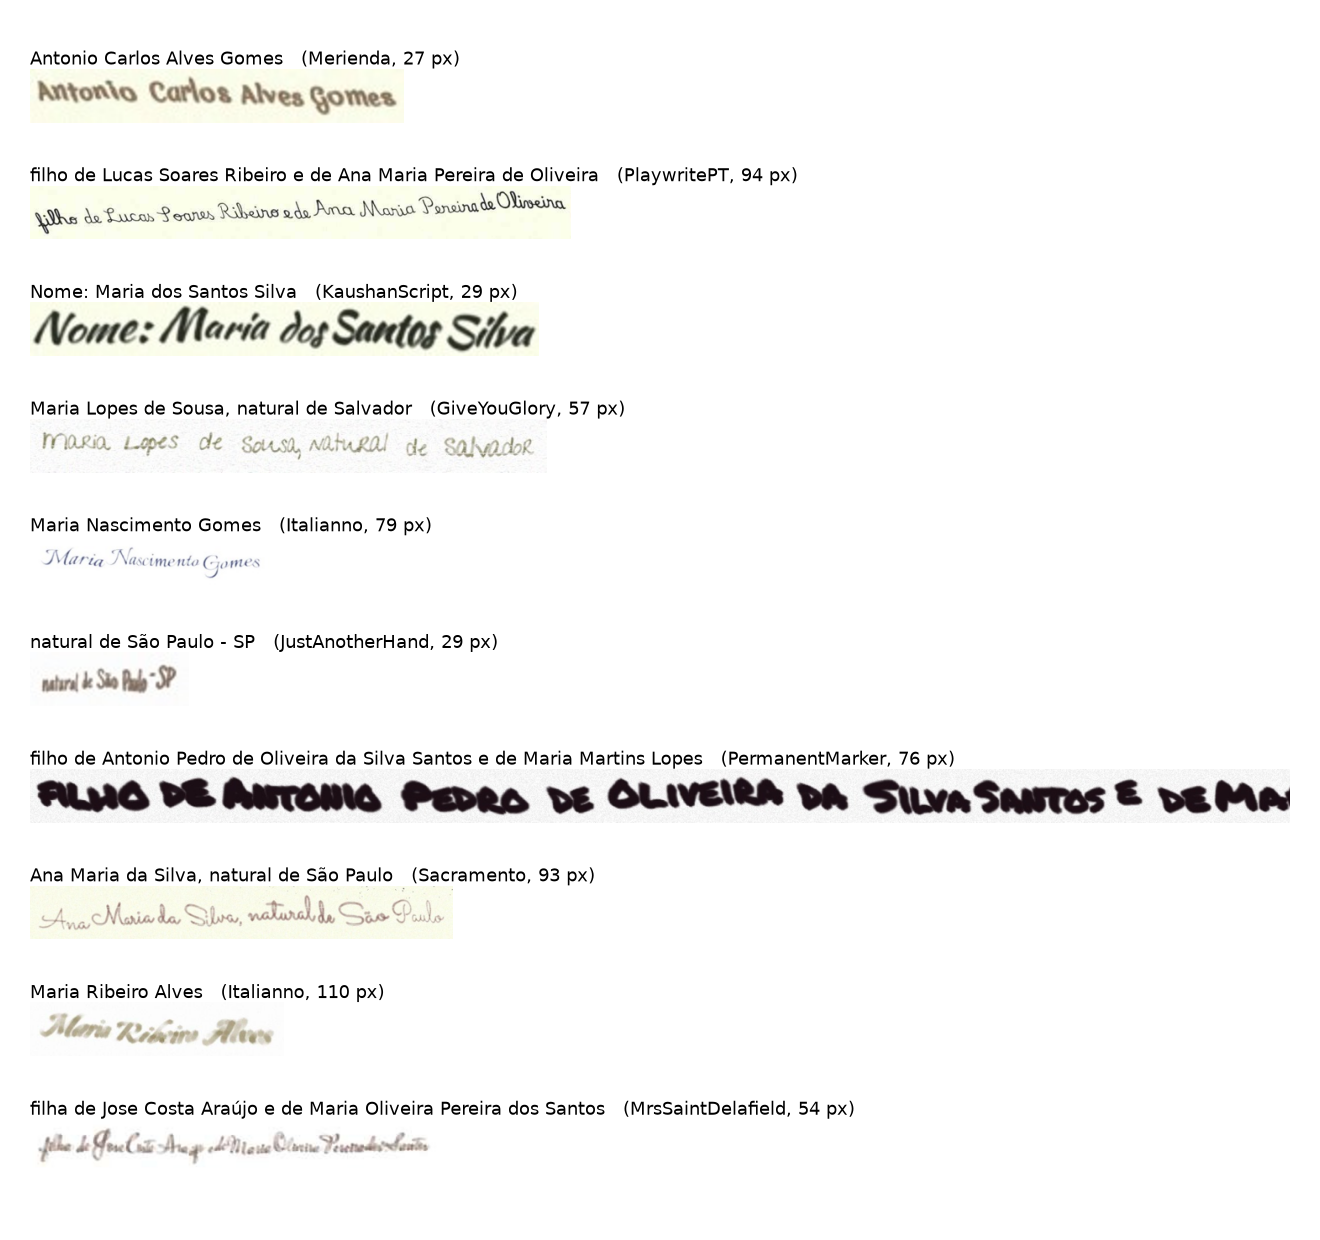
\includegraphics[width=0.7\textwidth]{figuras/exemplos_sinteticos_v2.png}
\caption{Linhas sintéticas como o modelo as recebe (64~px de altura), com o rótulo, a fonte e a altura gerada acima de cada uma.}
\label{fig:exemplos-v2}
\end{figure}

\begin{table}[H]
\centering
\small
\begin{tabular}{@{}llrrrrrr@{}}
\toprule
Modelo & \emph{Prompt} & CER & WER & Linhas exatas & CER nomes & CER inéditos & Nomes exatos \\
\midrule
\multicolumn{8}{@{}l}{\textit{BRESSAY (5.146 linhas, autores fora do treino)}} \\
Chandra & nativo & 20,1 & 34,1 & 12,6 & 20,9 & 28,8 & 66,4 \\
Chandra & curto & 19,8 & 33,9 & 12,3 & 18,6 & 28,3 & 68,1 \\
Chandra FP8 & nativo & 20,2 & 34,4 & 12,6 & 20,4 & 30,1 & 68,1 \\
Chandra FP8 & curto & 21,0 & 35,6 & 12,2 & 19,1 & 27,0 & 68,2 \\
lora\_v0 & nativo & \textbf{4,9} & 11,6 & 33,5 & 10,9 & 21,7 & 79,0 \\
lora\_v0 & curto & \textbf{4,9} & 11,5 & 33,5 & 11,0 & 21,2 & 78,4 \\
lora\_v0 FP8 & nativo & 5,0 & 11,7 & 33,2 & 10,7 & 24,3 & 79,1 \\
lora\_v0 FP8 & curto & 4,9 & 11,5 & 33,3 & 10,8 & 21,2 & 79,0 \\
\midrule
\multicolumn{8}{@{}l}{\textit{Sintético (4.000 linhas, 17 fontes e 8.508 nomes fora do treino)}} \\
Chandra & nativo & 8,6 & 21,4 & 47,2 & 8,6 & 9,4 & 74,6 \\
Chandra & curto & 6,2 & 18,8 & 49,0 & 8,0 & 8,9 & 75,8 \\
Chandra FP8 & nativo & 9,5 & 21,9 & 47,2 & 9,0 & 9,4 & 74,6 \\
Chandra FP8 & curto & 6,4 & 19,1 & 48,5 & 8,3 & 9,2 & 75,6 \\
lora\_v0 & nativo & 3,4 & 10,7 & 65,5 & 4,7 & 5,5 & 83,6 \\
lora\_v0 & curto & \textbf{3,3} & 10,6 & 65,7 & 4,7 & 5,5 & 83,7 \\
lora\_v0 FP8 & nativo & 3,4 & 10,7 & 65,3 & 4,7 & 5,5 & 83,5 \\
lora\_v0 FP8 & curto & 3,4 & 10,7 & 65,5 & 4,7 & 5,6 & 83,5 \\
\bottomrule
\end{tabular}
\caption{Resultados em linhas, em \%. Linhas exatas é a fração de linhas transcritas sem nenhum erro, e CER inéditos é o CER apenas nos nomes ausentes do treino (8.508 no sintético e 38 no BRESSAY).}
\label{tab:linhas-completa}
\end{table}

\begin{table}[H]
\centering
\small
\begin{tabular}{@{}llrrrr@{}}
\toprule
Modelo & & & CER & CER & Linhas erradas \\
(\emph{prompt} curto) & Teste & Marcadas & marcadas & não marcadas & marcadas \\
\midrule
Chandra & BRESSAY & 97,9\% & 20,0\% & 6,4\% & 98,8\% \\
Chandra & Sintético & 46,9\% & 10,5\% & 1,2\% & 74,0\% \\
lora\_v0 & BRESSAY & 56,9\% & 7,6\% & 1,0\% & 75,5\% \\
lora\_v0 & Sintético & 27,8\% & 8,7\% & 0,7\% & 68,4\% \\
\bottomrule
\end{tabular}
\caption{Linhas encaminhadas para revisão pelo \texttt{guard.py}. Linhas erradas marcadas é a fração das linhas com algum erro que foram para revisão. No modelo original, quase todas as linhas do BRESSAY foram marcadas por conterem HTML em resposta a um \emph{prompt} que pede texto puro.}
\label{tab:guard}
\end{table}

% --------------------------------------------------------------
\section{Exemplos Adicionais de Resultados}
\label{app:exemplos}

Cada linha de predição gravada pelo \texttt{infer.py} tem o formato abaixo. Os dois exemplos são predições do lora\_v0 com o \emph{prompt} curto no teste sintético (o campo \texttt{entities} foi omitido). No primeiro, o modelo inseriu um acento inexistente no nome, e a palavra errada foi a única marcada para revisão; no segundo, a linha está correta e não foi marcada.

{\footnotesize
\begin{verbatim}
{"id": "test_0000032", "source": "sintetico",
 "text": "Celi Nalva Ogura Ovando", "pred": "Celi Nálva Ogura Ovando",
 "guard": {"revisao": true, "motivos": ["confianca"],
           "palavras_baixa_confianca": ["Nálva"],
           "confianca_min": 0.4088}}
{"id": "test_0000011", "source": "sintetico",
 "text": "NOME: LIVIA ROZINEIDE MIADA ACUÑA",
 "pred": "NOME: LIVIA ROZINEIDE MIADA ACUÑA",
 "guard": {"revisao": false, "motivos": [],
           "palavras_baixa_confianca": [],
           "confianca_min": 0.9793}}
\end{verbatim}
}

Em página, a saída do Chandra é uma sequência de blocos HTML. O trecho abaixo é a saída do lora\_v2 para o campo do declarante da certidão da Figura~\ref{fig:gerador}, com o valor manuscrito em itálico:

{\scriptsize
\begin{verbatim}
<div data-bbox="79 536 174 547" data-label="Text"><p>Nome do Declarante</p></div>
<div data-bbox="98 552 377 577" data-label="Text"><p><i>Claudemar Reis Scalabrin</i></p></div>
<div data-bbox="357 536 443 547" data-label="Text"><p>Existência de bens</p></div>
<div data-bbox="511 536 601 547" data-label="Text"><p>Existência de filhos</p></div>
\end{verbatim}
}

% --------------------------------------------------------------
\section{Código-fonte}
\label{app:codigo}

\url{https://github.com/gabriel-salmoria/ai-sec}
